% Options for packages loaded elsewhere
\PassOptionsToPackage{unicode}{hyperref}
\PassOptionsToPackage{hyphens}{url}
%
\documentclass[
]{article}
\usepackage{amsmath,amssymb}
\usepackage{iftex}
\ifPDFTeX
  \usepackage[T1]{fontenc}
  \usepackage[utf8]{inputenc}
  \usepackage{textcomp} % provide euro and other symbols
\else % if luatex or xetex
  \usepackage{unicode-math} % this also loads fontspec
  \defaultfontfeatures{Scale=MatchLowercase}
  \defaultfontfeatures[\rmfamily]{Ligatures=TeX,Scale=1}
\fi
\usepackage{lmodern}
\ifPDFTeX\else
  % xetex/luatex font selection
\fi
% Use upquote if available, for straight quotes in verbatim environments
\IfFileExists{upquote.sty}{\usepackage{upquote}}{}
\IfFileExists{microtype.sty}{% use microtype if available
  \usepackage[]{microtype}
  \UseMicrotypeSet[protrusion]{basicmath} % disable protrusion for tt fonts
}{}
\makeatletter
\@ifundefined{KOMAClassName}{% if non-KOMA class
  \IfFileExists{parskip.sty}{%
    \usepackage{parskip}
  }{% else
    \setlength{\parindent}{0pt}
    \setlength{\parskip}{6pt plus 2pt minus 1pt}}
}{% if KOMA class
  \KOMAoptions{parskip=half}}
\makeatother
\usepackage{xcolor}
\usepackage[margin=1in]{geometry}
\usepackage{color}
\usepackage{fancyvrb}
\newcommand{\VerbBar}{|}
\newcommand{\VERB}{\Verb[commandchars=\\\{\}]}
\DefineVerbatimEnvironment{Highlighting}{Verbatim}{commandchars=\\\{\}}
% Add ',fontsize=\small' for more characters per line
\usepackage{framed}
\definecolor{shadecolor}{RGB}{248,248,248}
\newenvironment{Shaded}{\begin{snugshade}}{\end{snugshade}}
\newcommand{\AlertTok}[1]{\textcolor[rgb]{0.94,0.16,0.16}{#1}}
\newcommand{\AnnotationTok}[1]{\textcolor[rgb]{0.56,0.35,0.01}{\textbf{\textit{#1}}}}
\newcommand{\AttributeTok}[1]{\textcolor[rgb]{0.13,0.29,0.53}{#1}}
\newcommand{\BaseNTok}[1]{\textcolor[rgb]{0.00,0.00,0.81}{#1}}
\newcommand{\BuiltInTok}[1]{#1}
\newcommand{\CharTok}[1]{\textcolor[rgb]{0.31,0.60,0.02}{#1}}
\newcommand{\CommentTok}[1]{\textcolor[rgb]{0.56,0.35,0.01}{\textit{#1}}}
\newcommand{\CommentVarTok}[1]{\textcolor[rgb]{0.56,0.35,0.01}{\textbf{\textit{#1}}}}
\newcommand{\ConstantTok}[1]{\textcolor[rgb]{0.56,0.35,0.01}{#1}}
\newcommand{\ControlFlowTok}[1]{\textcolor[rgb]{0.13,0.29,0.53}{\textbf{#1}}}
\newcommand{\DataTypeTok}[1]{\textcolor[rgb]{0.13,0.29,0.53}{#1}}
\newcommand{\DecValTok}[1]{\textcolor[rgb]{0.00,0.00,0.81}{#1}}
\newcommand{\DocumentationTok}[1]{\textcolor[rgb]{0.56,0.35,0.01}{\textbf{\textit{#1}}}}
\newcommand{\ErrorTok}[1]{\textcolor[rgb]{0.64,0.00,0.00}{\textbf{#1}}}
\newcommand{\ExtensionTok}[1]{#1}
\newcommand{\FloatTok}[1]{\textcolor[rgb]{0.00,0.00,0.81}{#1}}
\newcommand{\FunctionTok}[1]{\textcolor[rgb]{0.13,0.29,0.53}{\textbf{#1}}}
\newcommand{\ImportTok}[1]{#1}
\newcommand{\InformationTok}[1]{\textcolor[rgb]{0.56,0.35,0.01}{\textbf{\textit{#1}}}}
\newcommand{\KeywordTok}[1]{\textcolor[rgb]{0.13,0.29,0.53}{\textbf{#1}}}
\newcommand{\NormalTok}[1]{#1}
\newcommand{\OperatorTok}[1]{\textcolor[rgb]{0.81,0.36,0.00}{\textbf{#1}}}
\newcommand{\OtherTok}[1]{\textcolor[rgb]{0.56,0.35,0.01}{#1}}
\newcommand{\PreprocessorTok}[1]{\textcolor[rgb]{0.56,0.35,0.01}{\textit{#1}}}
\newcommand{\RegionMarkerTok}[1]{#1}
\newcommand{\SpecialCharTok}[1]{\textcolor[rgb]{0.81,0.36,0.00}{\textbf{#1}}}
\newcommand{\SpecialStringTok}[1]{\textcolor[rgb]{0.31,0.60,0.02}{#1}}
\newcommand{\StringTok}[1]{\textcolor[rgb]{0.31,0.60,0.02}{#1}}
\newcommand{\VariableTok}[1]{\textcolor[rgb]{0.00,0.00,0.00}{#1}}
\newcommand{\VerbatimStringTok}[1]{\textcolor[rgb]{0.31,0.60,0.02}{#1}}
\newcommand{\WarningTok}[1]{\textcolor[rgb]{0.56,0.35,0.01}{\textbf{\textit{#1}}}}
\usepackage{graphicx}
\makeatletter
\def\maxwidth{\ifdim\Gin@nat@width>\linewidth\linewidth\else\Gin@nat@width\fi}
\def\maxheight{\ifdim\Gin@nat@height>\textheight\textheight\else\Gin@nat@height\fi}
\makeatother
% Scale images if necessary, so that they will not overflow the page
% margins by default, and it is still possible to overwrite the defaults
% using explicit options in \includegraphics[width, height, ...]{}
\setkeys{Gin}{width=\maxwidth,height=\maxheight,keepaspectratio}
% Set default figure placement to htbp
\makeatletter
\def\fps@figure{htbp}
\makeatother
\setlength{\emergencystretch}{3em} % prevent overfull lines
\providecommand{\tightlist}{%
  \setlength{\itemsep}{0pt}\setlength{\parskip}{0pt}}
\setcounter{secnumdepth}{-\maxdimen} % remove section numbering
\ifLuaTeX
  \usepackage{selnolig}  % disable illegal ligatures
\fi
\IfFileExists{bookmark.sty}{\usepackage{bookmark}}{\usepackage{hyperref}}
\IfFileExists{xurl.sty}{\usepackage{xurl}}{} % add URL line breaks if available
\urlstyle{same}
\hypersetup{
  pdftitle={Challenge 7},
  pdfauthor={Ariel Quek},
  hidelinks,
  pdfcreator={LaTeX via pandoc}}

\title{Challenge 7}
\author{Ariel Quek}
\date{2023-10-02}

\begin{document}
\maketitle

\begin{Shaded}
\begin{Highlighting}[]
\NormalTok{knitr}\SpecialCharTok{::}\NormalTok{opts\_chunk}\SpecialCharTok{$}\FunctionTok{set}\NormalTok{(}\AttributeTok{echo =} \ConstantTok{TRUE}\NormalTok{)}
\end{Highlighting}
\end{Shaded}

\hypertarget{challenge-7-instructions}{%
\subsection{Challenge 7 Instructions}\label{challenge-7-instructions}}

\begin{enumerate}
\def\labelenumi{\arabic{enumi}.}
\item
  You are required to focus on the lecture videos and materials, owing
  to the break last week
\item
  The material taught this week is of significant importance for your
  final projects
\item
  The challenge this week will be your workbook: a document that you
  will generate by trying and experimenting with the code snippets
  taught in the lecture material.
\end{enumerate}

\begin{Shaded}
\begin{Highlighting}[]
\FunctionTok{library}\NormalTok{(tidyverse)}
\end{Highlighting}
\end{Shaded}

\begin{verbatim}
## -- Attaching core tidyverse packages ------------------------ tidyverse 2.0.0 --
## v dplyr     1.1.0     v readr     2.1.4
## v forcats   1.0.0     v stringr   1.5.0
## v ggplot2   3.4.3     v tibble    3.1.8
## v lubridate 1.9.2     v tidyr     1.3.0
## v purrr     1.0.1     
## -- Conflicts ------------------------------------------ tidyverse_conflicts() --
## x dplyr::filter() masks stats::filter()
## x dplyr::lag()    masks stats::lag()
## i Use the ]8;;http://conflicted.r-lib.org/conflicted package]8;; to force all conflicts to become errors
\end{verbatim}

\begin{Shaded}
\begin{Highlighting}[]
\FunctionTok{install.packages}\NormalTok{(}\StringTok{"palmerpenguins"}\NormalTok{,}\AttributeTok{repos =} \StringTok{"http://cran.us.r{-}project.org"}\NormalTok{)}
\end{Highlighting}
\end{Shaded}

\begin{verbatim}
## Installing package into 'C:/Users/Ariel/AppData/Local/R/win-library/4.2'
## (as 'lib' is unspecified)
\end{verbatim}

\begin{verbatim}
## package 'palmerpenguins' successfully unpacked and MD5 sums checked
## 
## The downloaded binary packages are in
##  C:\Users\Ariel\AppData\Local\Temp\RtmpAN6bmy\downloaded_packages
\end{verbatim}

\begin{Shaded}
\begin{Highlighting}[]
\FunctionTok{library}\NormalTok{(palmerpenguins)}
\FunctionTok{glimpse}\NormalTok{(penguins)}
\end{Highlighting}
\end{Shaded}

\begin{verbatim}
## Rows: 344
## Columns: 8
## $ species           <fct> Adelie, Adelie, Adelie, Adelie, Adelie, Adelie, Adel~
## $ island            <fct> Torgersen, Torgersen, Torgersen, Torgersen, Torgerse~
## $ bill_length_mm    <dbl> 39.1, 39.5, 40.3, NA, 36.7, 39.3, 38.9, 39.2, 34.1, ~
## $ bill_depth_mm     <dbl> 18.7, 17.4, 18.0, NA, 19.3, 20.6, 17.8, 19.6, 18.1, ~
## $ flipper_length_mm <int> 181, 186, 195, NA, 193, 190, 181, 195, 193, 190, 186~
## $ body_mass_g       <int> 3750, 3800, 3250, NA, 3450, 3650, 3625, 4675, 3475, ~
## $ sex               <fct> male, female, female, NA, female, male, female, male~
## $ year              <int> 2007, 2007, 2007, 2007, 2007, 2007, 2007, 2007, 2007~
\end{verbatim}

\hypertarget{recreating-plot-for-palmer-penguins}{%
\subsection{Recreating Plot for Palmer
Penguins}\label{recreating-plot-for-palmer-penguins}}

Plotting the bill depth against bill length of penguins

\begin{Shaded}
\begin{Highlighting}[]
\FunctionTok{ggplot}\NormalTok{(}\AttributeTok{data =}\NormalTok{ penguins,}
       \AttributeTok{mapping =} \FunctionTok{aes}\NormalTok{(}\AttributeTok{x =}\NormalTok{ bill\_depth\_mm,}
                     \AttributeTok{y =}\NormalTok{ bill\_length\_mm,}
                     \AttributeTok{colour =}\NormalTok{ species))}\SpecialCharTok{+}
  \FunctionTok{geom\_point}\NormalTok{() }\SpecialCharTok{+}
  \FunctionTok{labs}\NormalTok{(}\AttributeTok{title =} \StringTok{"Bill depth and length"}\NormalTok{, }
       \AttributeTok{subtitle =} \StringTok{"Dimensions for Adelie, Chinstrap, and Gentoo Penguins"}\NormalTok{,}
       \AttributeTok{x =}\StringTok{"Bill depth (mm)"}\NormalTok{, }
       \AttributeTok{y =} \StringTok{"Bill length (mm)"}\NormalTok{,}
       \AttributeTok{colour =} \StringTok{"Species"}\NormalTok{,}
       \AttributeTok{caption =} \StringTok{"Source: Palmer Station LTER/ palmerpenguins package"}\NormalTok{,}
\FunctionTok{scale\_colour\_viridis\_d}\NormalTok{())}
\end{Highlighting}
\end{Shaded}

\begin{verbatim}
## Warning: Removed 2 rows containing missing values (`geom_point()`).
\end{verbatim}

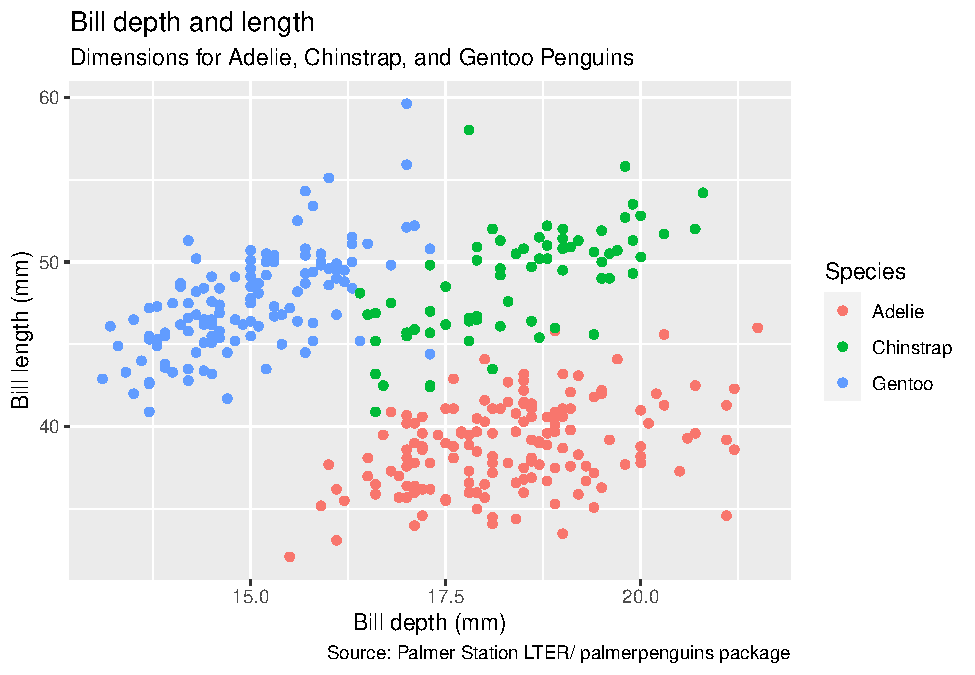
\includegraphics{Challenge-7-File_files/figure-latex/unnamed-chunk-2-1.pdf}
Plotting bill depth against bill length with shaped data points:

\begin{Shaded}
\begin{Highlighting}[]
\FunctionTok{ggplot}\NormalTok{(penguins, }\FunctionTok{aes}\NormalTok{(}\AttributeTok{x =}\NormalTok{ bill\_depth\_mm, }\AttributeTok{y =}\NormalTok{ bill\_length\_mm, }\AttributeTok{colour =}\NormalTok{ species,}
\AttributeTok{shape =}\NormalTok{ island)) }\SpecialCharTok{+}
\FunctionTok{geom\_point}\NormalTok{() }\SpecialCharTok{+} \FunctionTok{scale\_colour\_viridis\_d}\NormalTok{()}
\end{Highlighting}
\end{Shaded}

\begin{verbatim}
## Warning: Removed 2 rows containing missing values (`geom_point()`).
\end{verbatim}

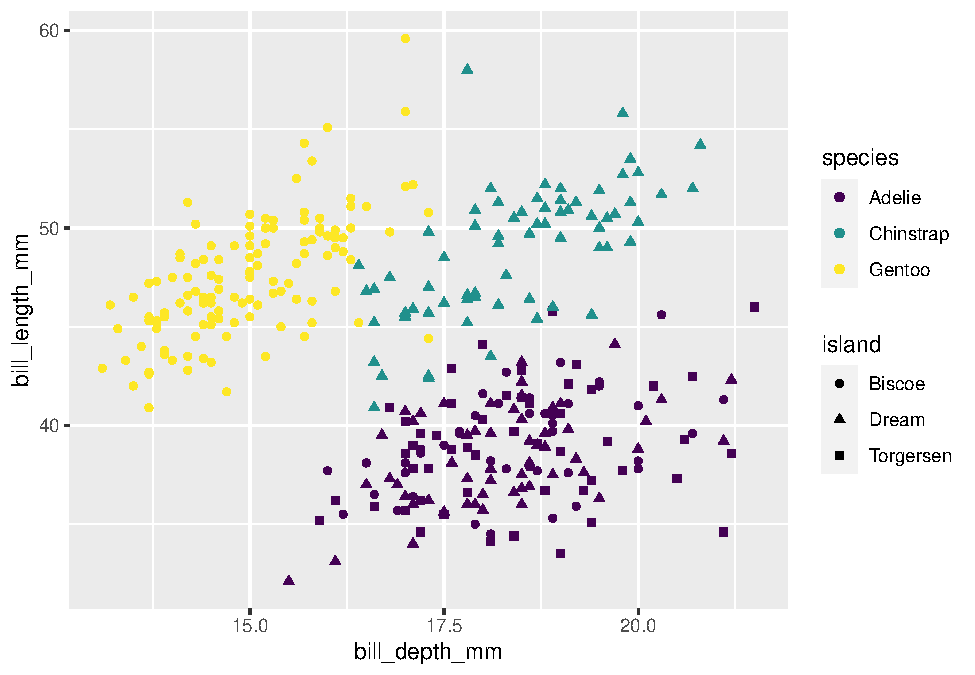
\includegraphics{Challenge-7-File_files/figure-latex/unnamed-chunk-3-1.pdf}

Changing the size of data points on the plot

\begin{Shaded}
\begin{Highlighting}[]
\FunctionTok{ggplot}\NormalTok{(penguins, }\FunctionTok{aes}\NormalTok{(}\AttributeTok{x =}\NormalTok{ bill\_depth\_mm, }\AttributeTok{y =}\NormalTok{ bill\_length\_mm, }\AttributeTok{colour =}\NormalTok{ species, }\AttributeTok{shape =}\NormalTok{ species,}
\AttributeTok{size =}\NormalTok{ body\_mass\_g)) }\SpecialCharTok{+}
\FunctionTok{geom\_point}\NormalTok{() }\SpecialCharTok{+} \FunctionTok{scale\_colour\_viridis\_d}\NormalTok{()}
\end{Highlighting}
\end{Shaded}

\begin{verbatim}
## Warning: Removed 2 rows containing missing values (`geom_point()`).
\end{verbatim}

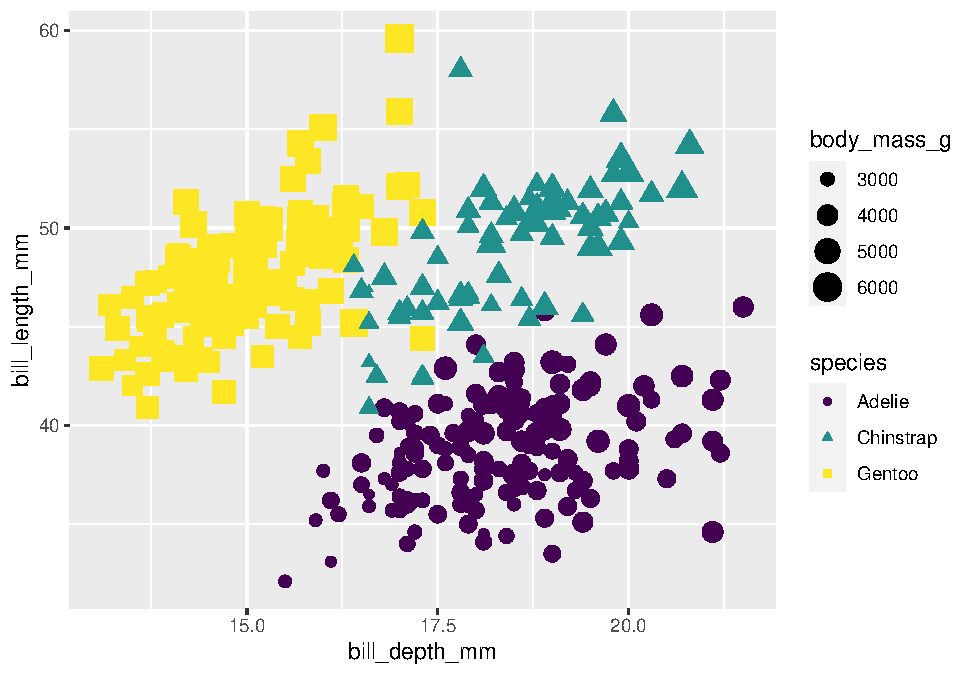
\includegraphics{Challenge-7-File_files/figure-latex/unnamed-chunk-4-1.pdf}

Manipulating alpha (opacity) of data points in the plot

\begin{Shaded}
\begin{Highlighting}[]
\FunctionTok{ggplot}\NormalTok{(penguins, }\FunctionTok{aes}\NormalTok{(}\AttributeTok{x =}\NormalTok{ bill\_depth\_mm, }\AttributeTok{y =}\NormalTok{ bill\_length\_mm, }\AttributeTok{colour =}\NormalTok{ species,}
\AttributeTok{shape =}\NormalTok{ species, }\AttributeTok{size =}\NormalTok{ body\_mass\_g, }\AttributeTok{alpha =}\NormalTok{ flipper\_length\_mm)) }\SpecialCharTok{+}
\FunctionTok{geom\_point}\NormalTok{() }\SpecialCharTok{+} \FunctionTok{scale\_colour\_viridis\_d}\NormalTok{()}
\end{Highlighting}
\end{Shaded}

\begin{verbatim}
## Warning: Removed 2 rows containing missing values (`geom_point()`).
\end{verbatim}

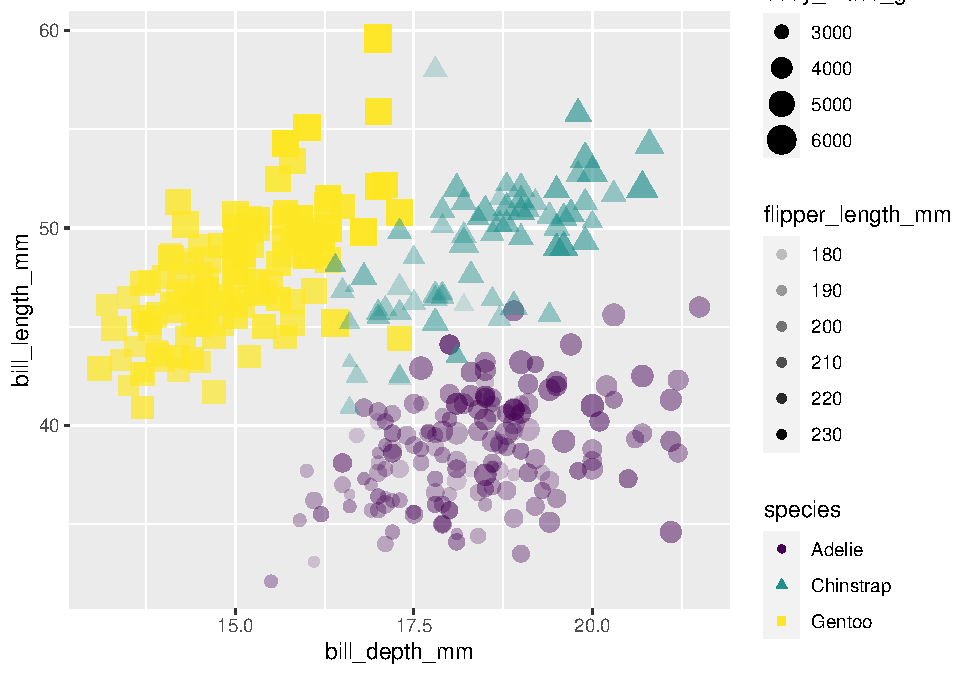
\includegraphics{Challenge-7-File_files/figure-latex/unnamed-chunk-5-1.pdf}

\hypertarget{faceting-creating-smaller-plots-that-display-different-subsets-of-the-data}{%
\subsection{Faceting: creating smaller plots that display different
subsets of the
data}\label{faceting-creating-smaller-plots-that-display-different-subsets-of-the-data}}

\emph{1. Plotting the bill length and bill depth of penguins based on
the species and the island}

\begin{Shaded}
\begin{Highlighting}[]
\FunctionTok{ggplot}\NormalTok{(penguins) }\SpecialCharTok{+}
\FunctionTok{aes}\NormalTok{(}\AttributeTok{x =}\NormalTok{ bill\_depth\_mm,}
\AttributeTok{y =}\NormalTok{ bill\_length\_mm) }\SpecialCharTok{+}
\FunctionTok{geom\_point}\NormalTok{() }\SpecialCharTok{+}
\FunctionTok{facet\_grid}\NormalTok{(species }\SpecialCharTok{\textasciitilde{}}\NormalTok{ island)}
\end{Highlighting}
\end{Shaded}

\begin{verbatim}
## Warning: Removed 2 rows containing missing values (`geom_point()`).
\end{verbatim}

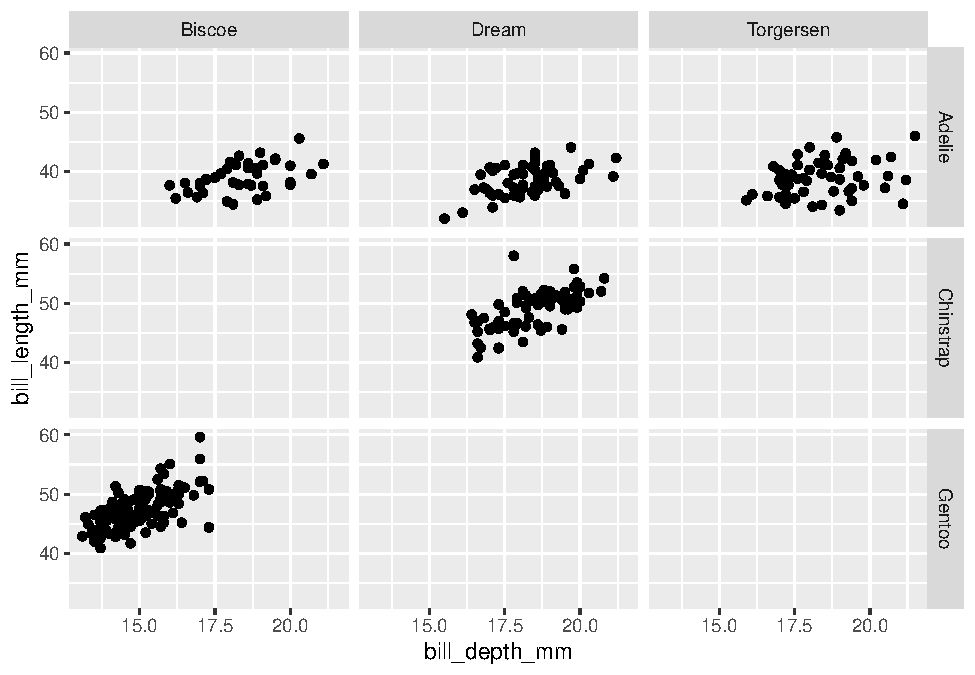
\includegraphics{Challenge-7-File_files/figure-latex/unnamed-chunk-6-1.pdf}

\emph{2. Plotting bill length and bill depth of penguins based on sex
against species}

\begin{Shaded}
\begin{Highlighting}[]
\FunctionTok{ggplot}\NormalTok{(penguins, }\FunctionTok{aes}\NormalTok{(}\AttributeTok{x =}\NormalTok{ bill\_depth\_mm, }\AttributeTok{y =}\NormalTok{ bill\_length\_mm)) }\SpecialCharTok{+} \FunctionTok{geom\_point}\NormalTok{() }\SpecialCharTok{+}
\FunctionTok{facet\_grid}\NormalTok{(species }\SpecialCharTok{\textasciitilde{}}\NormalTok{ sex)}
\end{Highlighting}
\end{Shaded}

\begin{verbatim}
## Warning: Removed 2 rows containing missing values (`geom_point()`).
\end{verbatim}

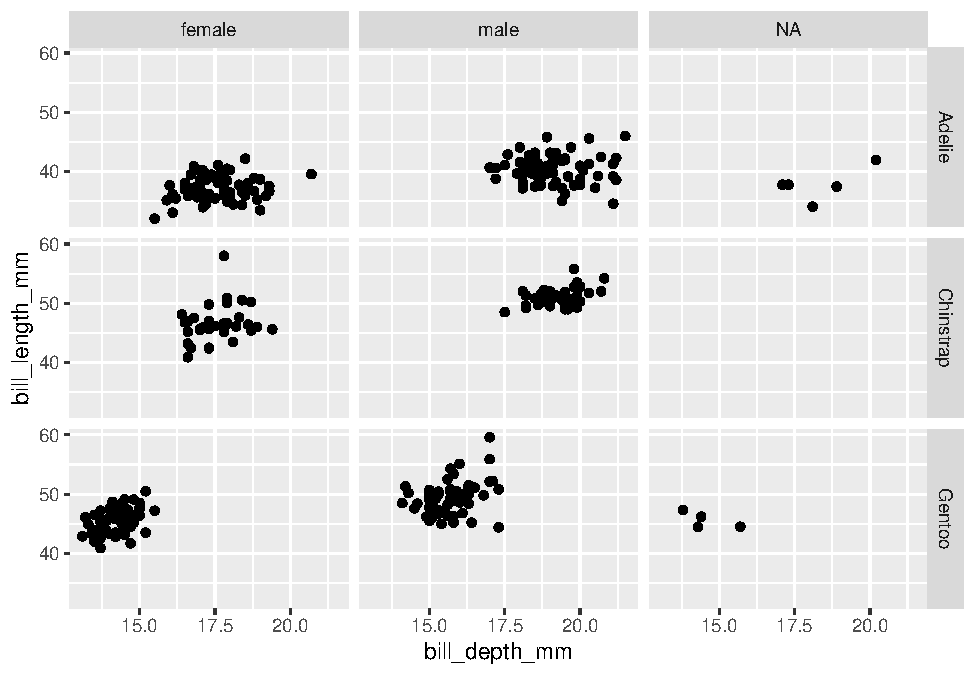
\includegraphics{Challenge-7-File_files/figure-latex/unnamed-chunk-7-1.pdf}

\emph{3. Alternatively, plotting bill length and bill depth of penguins
based on species against sex}

\begin{Shaded}
\begin{Highlighting}[]
\FunctionTok{ggplot}\NormalTok{(penguins, }\FunctionTok{aes}\NormalTok{(}\AttributeTok{x =}\NormalTok{ bill\_depth\_mm, }\AttributeTok{y =}\NormalTok{ bill\_length\_mm)) }\SpecialCharTok{+} \FunctionTok{geom\_point}\NormalTok{() }\SpecialCharTok{+}
\FunctionTok{facet\_grid}\NormalTok{(sex }\SpecialCharTok{\textasciitilde{}}\NormalTok{ species)}
\end{Highlighting}
\end{Shaded}

\begin{verbatim}
## Warning: Removed 2 rows containing missing values (`geom_point()`).
\end{verbatim}

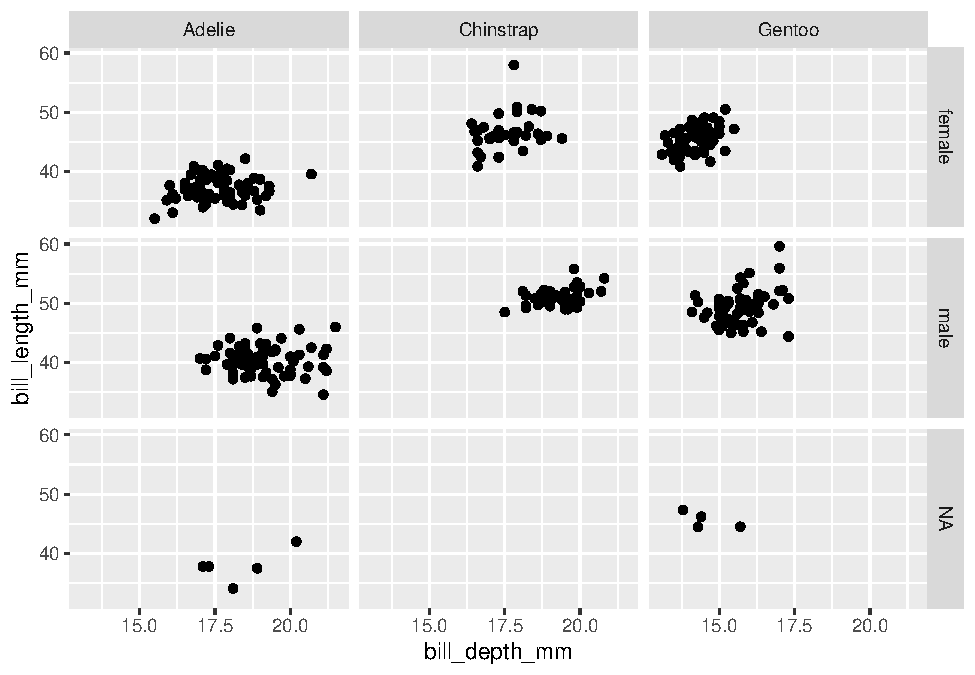
\includegraphics{Challenge-7-File_files/figure-latex/unnamed-chunk-8-1.pdf}

\emph{4. Plotting bill length against bill depth only by species}

\begin{Shaded}
\begin{Highlighting}[]
\FunctionTok{ggplot}\NormalTok{(penguins, }\FunctionTok{aes}\NormalTok{(}\AttributeTok{x =}\NormalTok{ bill\_depth\_mm, }\AttributeTok{y =}\NormalTok{ bill\_length\_mm)) }\SpecialCharTok{+} \FunctionTok{geom\_point}\NormalTok{() }\SpecialCharTok{+}
\FunctionTok{facet\_wrap}\NormalTok{(}\SpecialCharTok{\textasciitilde{}}\NormalTok{ species)}
\end{Highlighting}
\end{Shaded}

\begin{verbatim}
## Warning: Removed 2 rows containing missing values (`geom_point()`).
\end{verbatim}

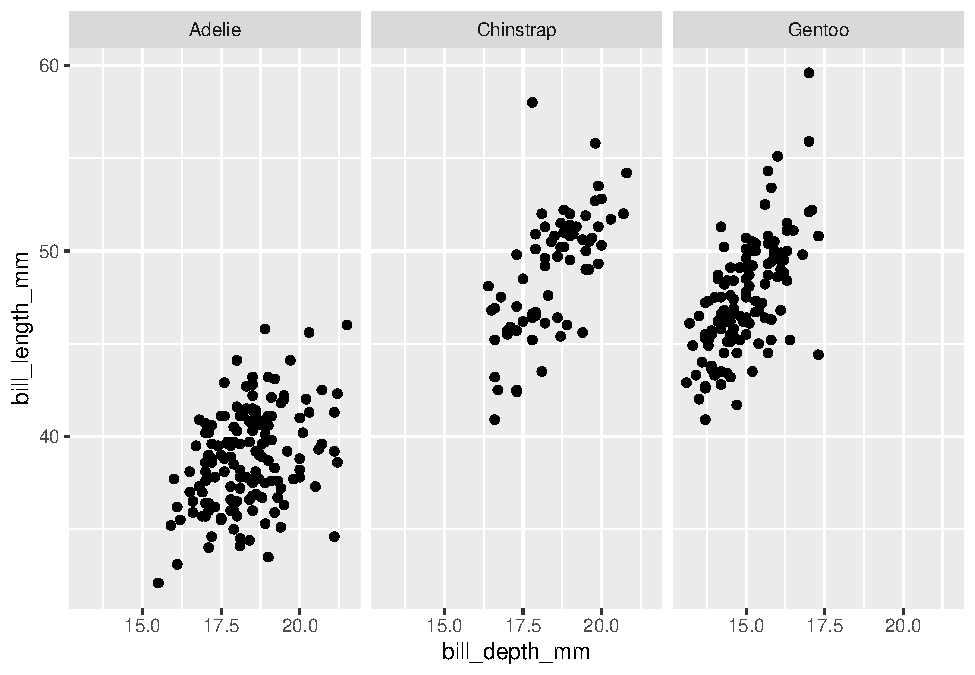
\includegraphics{Challenge-7-File_files/figure-latex/unnamed-chunk-9-1.pdf}
\emph{5. Plotting bill length against bill depth by species, in separate
grids}

\begin{Shaded}
\begin{Highlighting}[]
\FunctionTok{ggplot}\NormalTok{(penguins, }\FunctionTok{aes}\NormalTok{(}\AttributeTok{x =}\NormalTok{ bill\_depth\_mm, }\AttributeTok{y =}\NormalTok{ bill\_length\_mm)) }\SpecialCharTok{+} \FunctionTok{geom\_point}\NormalTok{()}\SpecialCharTok{+}
\FunctionTok{facet\_wrap}\NormalTok{(}\SpecialCharTok{\textasciitilde{}}\NormalTok{ species, }\AttributeTok{ncol =}\DecValTok{2}\NormalTok{)}
\end{Highlighting}
\end{Shaded}

\begin{verbatim}
## Warning: Removed 2 rows containing missing values (`geom_point()`).
\end{verbatim}

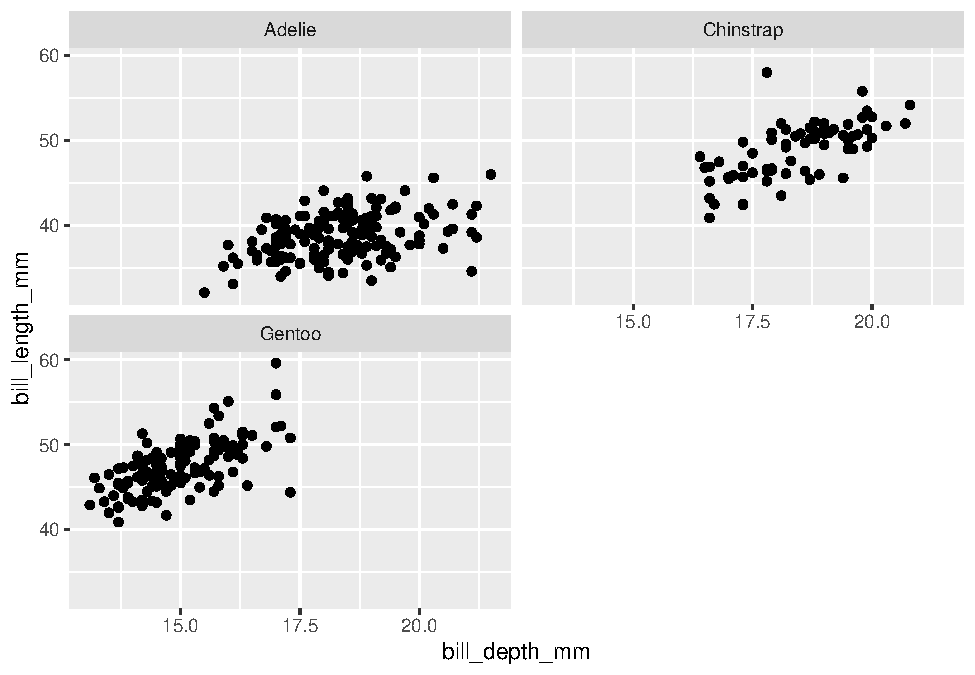
\includegraphics{Challenge-7-File_files/figure-latex/unnamed-chunk-10-1.pdf}
\emph{6. Adding colour (without a legend)}

\begin{Shaded}
\begin{Highlighting}[]
\FunctionTok{ggplot}\NormalTok{(penguins, }\FunctionTok{aes}\NormalTok{(}\AttributeTok{x =}\NormalTok{ bill\_depth\_mm, }\AttributeTok{y =}\NormalTok{ bill\_length\_mm, }\AttributeTok{color =}\NormalTok{ species)) }\SpecialCharTok{+}
\FunctionTok{geom\_point}\NormalTok{() }\SpecialCharTok{+} \FunctionTok{facet\_grid}\NormalTok{(species }\SpecialCharTok{\textasciitilde{}}\NormalTok{ sex) }\SpecialCharTok{+} \FunctionTok{scale\_color\_viridis\_d}\NormalTok{() }\SpecialCharTok{+}
\FunctionTok{guides}\NormalTok{(}\AttributeTok{color =}
\StringTok{"none"}
\NormalTok{)}
\end{Highlighting}
\end{Shaded}

\begin{verbatim}
## Warning: Removed 2 rows containing missing values (`geom_point()`).
\end{verbatim}

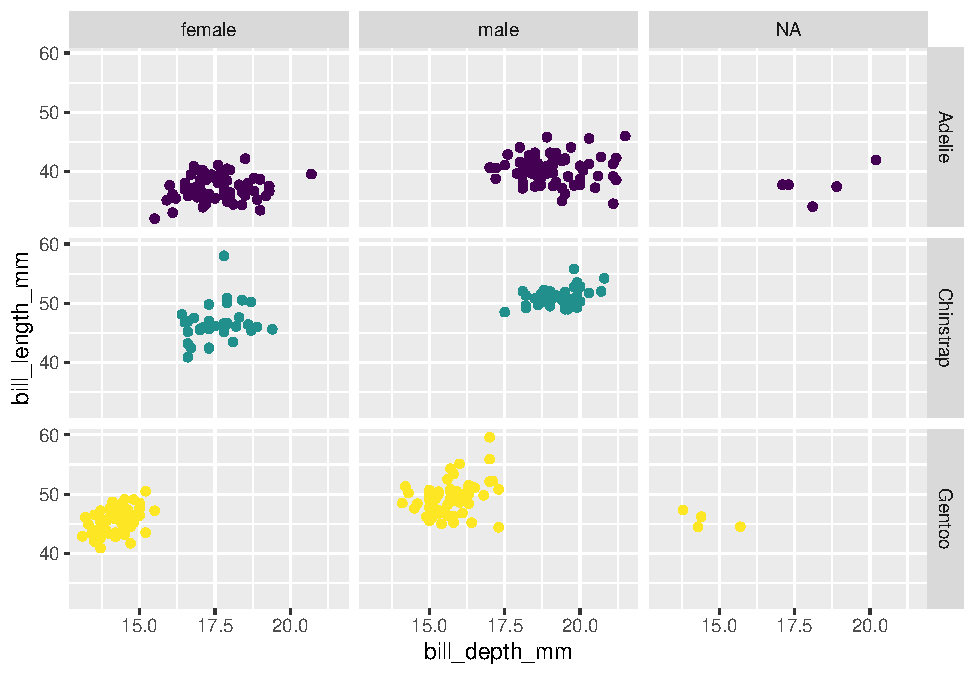
\includegraphics{Challenge-7-File_files/figure-latex/unnamed-chunk-11-1.pdf}
\#\# Visualizing numeric variables using Lending Club Data set

Retrieving dataset

\begin{Shaded}
\begin{Highlighting}[]
\FunctionTok{install.packages}\NormalTok{(}\StringTok{"openintro"}\NormalTok{, }\AttributeTok{repos =} \StringTok{"http://cran.us.r{-}project.org"}\NormalTok{)}
\end{Highlighting}
\end{Shaded}

\begin{verbatim}
## Installing package into 'C:/Users/Ariel/AppData/Local/R/win-library/4.2'
## (as 'lib' is unspecified)
\end{verbatim}

\begin{verbatim}
## Warning in download.file(url, destfile, method, mode = "wb", ...): URL
## 'http://cran.us.r-project.org/bin/windows/contrib/4.2/openintro_2.4.0.zip':
## Timeout of 60 seconds was reached
\end{verbatim}

\begin{verbatim}
## Error in download.file(url, destfile, method, mode = "wb", ...) : 
##   cannot open URL 'http://cran.us.r-project.org/bin/windows/contrib/4.2/openintro_2.4.0.zip'
\end{verbatim}

\begin{verbatim}
## Warning in download.packages(pkgs, destdir = tmpd, available = available, :
## download of package 'openintro' failed
\end{verbatim}

\begin{Shaded}
\begin{Highlighting}[]
\FunctionTok{library}\NormalTok{(openintro)}
\end{Highlighting}
\end{Shaded}

\begin{verbatim}
## Warning: package 'openintro' was built under R version 4.2.3
\end{verbatim}

\begin{verbatim}
## Loading required package: airports
\end{verbatim}

\begin{verbatim}
## Warning: package 'airports' was built under R version 4.2.3
\end{verbatim}

\begin{verbatim}
## Loading required package: cherryblossom
\end{verbatim}

\begin{verbatim}
## Warning: package 'cherryblossom' was built under R version 4.2.3
\end{verbatim}

\begin{verbatim}
## Loading required package: usdata
\end{verbatim}

\begin{verbatim}
## Warning: package 'usdata' was built under R version 4.2.3
\end{verbatim}

\begin{Shaded}
\begin{Highlighting}[]
\FunctionTok{library}\NormalTok{(tidyverse)}
\FunctionTok{glimpse}\NormalTok{(loans\_full\_schema)}
\end{Highlighting}
\end{Shaded}

\begin{verbatim}
## Rows: 10,000
## Columns: 55
## $ emp_title                        <chr> "global config engineer ", "warehouse~
## $ emp_length                       <dbl> 3, 10, 3, 1, 10, NA, 10, 10, 10, 3, 1~
## $ state                            <fct> NJ, HI, WI, PA, CA, KY, MI, AZ, NV, I~
## $ homeownership                    <fct> MORTGAGE, RENT, RENT, RENT, RENT, OWN~
## $ annual_income                    <dbl> 90000, 40000, 40000, 30000, 35000, 34~
## $ verified_income                  <fct> Verified, Not Verified, Source Verifi~
## $ debt_to_income                   <dbl> 18.01, 5.04, 21.15, 10.16, 57.96, 6.4~
## $ annual_income_joint              <dbl> NA, NA, NA, NA, 57000, NA, 155000, NA~
## $ verification_income_joint        <fct> , , , , Verified, , Not Verified, , ,~
## $ debt_to_income_joint             <dbl> NA, NA, NA, NA, 37.66, NA, 13.12, NA,~
## $ delinq_2y                        <int> 0, 0, 0, 0, 0, 1, 0, 1, 1, 0, 0, 0, 0~
## $ months_since_last_delinq         <int> 38, NA, 28, NA, NA, 3, NA, 19, 18, NA~
## $ earliest_credit_line             <dbl> 2001, 1996, 2006, 2007, 2008, 1990, 2~
## $ inquiries_last_12m               <int> 6, 1, 4, 0, 7, 6, 1, 1, 3, 0, 4, 4, 8~
## $ total_credit_lines               <int> 28, 30, 31, 4, 22, 32, 12, 30, 35, 9,~
## $ open_credit_lines                <int> 10, 14, 10, 4, 16, 12, 10, 15, 21, 6,~
## $ total_credit_limit               <int> 70795, 28800, 24193, 25400, 69839, 42~
## $ total_credit_utilized            <int> 38767, 4321, 16000, 4997, 52722, 3898~
## $ num_collections_last_12m         <int> 0, 0, 0, 0, 0, 0, 0, 0, 0, 0, 0, 0, 0~
## $ num_historical_failed_to_pay     <int> 0, 1, 0, 1, 0, 0, 0, 0, 0, 0, 1, 0, 0~
## $ months_since_90d_late            <int> 38, NA, 28, NA, NA, 60, NA, 71, 18, N~
## $ current_accounts_delinq          <int> 0, 0, 0, 0, 0, 0, 0, 0, 0, 0, 0, 0, 0~
## $ total_collection_amount_ever     <int> 1250, 0, 432, 0, 0, 0, 0, 0, 0, 0, 0,~
## $ current_installment_accounts     <int> 2, 0, 1, 1, 1, 0, 2, 2, 6, 1, 2, 1, 2~
## $ accounts_opened_24m              <int> 5, 11, 13, 1, 6, 2, 1, 4, 10, 5, 6, 7~
## $ months_since_last_credit_inquiry <int> 5, 8, 7, 15, 4, 5, 9, 7, 4, 17, 3, 4,~
## $ num_satisfactory_accounts        <int> 10, 14, 10, 4, 16, 12, 10, 15, 21, 6,~
## $ num_accounts_120d_past_due       <int> 0, 0, 0, 0, 0, 0, 0, NA, 0, 0, 0, 0, ~
## $ num_accounts_30d_past_due        <int> 0, 0, 0, 0, 0, 0, 0, 0, 0, 0, 0, 0, 0~
## $ num_active_debit_accounts        <int> 2, 3, 3, 2, 10, 1, 3, 5, 11, 3, 2, 2,~
## $ total_debit_limit                <int> 11100, 16500, 4300, 19400, 32700, 272~
## $ num_total_cc_accounts            <int> 14, 24, 14, 3, 20, 27, 8, 16, 19, 7, ~
## $ num_open_cc_accounts             <int> 8, 14, 8, 3, 15, 12, 7, 12, 14, 5, 8,~
## $ num_cc_carrying_balance          <int> 6, 4, 6, 2, 13, 5, 6, 10, 14, 3, 5, 3~
## $ num_mort_accounts                <int> 1, 0, 0, 0, 0, 3, 2, 7, 2, 0, 2, 3, 3~
## $ account_never_delinq_percent     <dbl> 92.9, 100.0, 93.5, 100.0, 100.0, 78.1~
## $ tax_liens                        <int> 0, 0, 0, 1, 0, 0, 0, 0, 0, 0, 0, 0, 0~
## $ public_record_bankrupt           <int> 0, 1, 0, 0, 0, 0, 0, 0, 0, 0, 1, 0, 0~
## $ loan_purpose                     <fct> moving, debt_consolidation, other, de~
## $ application_type                 <fct> individual, individual, individual, i~
## $ loan_amount                      <int> 28000, 5000, 2000, 21600, 23000, 5000~
## $ term                             <dbl> 60, 36, 36, 36, 36, 36, 60, 60, 36, 3~
## $ interest_rate                    <dbl> 14.07, 12.61, 17.09, 6.72, 14.07, 6.7~
## $ installment                      <dbl> 652.53, 167.54, 71.40, 664.19, 786.87~
## $ grade                            <fct> C, C, D, A, C, A, C, B, C, A, C, B, C~
## $ sub_grade                        <fct> C3, C1, D1, A3, C3, A3, C2, B5, C2, A~
## $ issue_month                      <fct> Mar-2018, Feb-2018, Feb-2018, Jan-201~
## $ loan_status                      <fct> Current, Current, Current, Current, C~
## $ initial_listing_status           <fct> whole, whole, fractional, whole, whol~
## $ disbursement_method              <fct> Cash, Cash, Cash, Cash, Cash, Cash, C~
## $ balance                          <dbl> 27015.86, 4651.37, 1824.63, 18853.26,~
## $ paid_total                       <dbl> 1999.330, 499.120, 281.800, 3312.890,~
## $ paid_principal                   <dbl> 984.14, 348.63, 175.37, 2746.74, 1569~
## $ paid_interest                    <dbl> 1015.19, 150.49, 106.43, 566.15, 754.~
## $ paid_late_fees                   <dbl> 0, 0, 0, 0, 0, 0, 0, 0, 0, 0, 0, 0, 0~
\end{verbatim}

Selecting variables

\begin{Shaded}
\begin{Highlighting}[]
\NormalTok{loans }\OtherTok{\textless{}{-}}\NormalTok{ loans\_full\_schema }\SpecialCharTok{\%\textgreater{}\%}
\FunctionTok{select}\NormalTok{(loan\_amount, interest\_rate, term, grade,}
\NormalTok{state, annual\_income, homeownership, debt\_to\_income)}
\FunctionTok{glimpse}\NormalTok{(loans)}
\end{Highlighting}
\end{Shaded}

\begin{verbatim}
## Rows: 10,000
## Columns: 8
## $ loan_amount    <int> 28000, 5000, 2000, 21600, 23000, 5000, 24000, 20000, 20~
## $ interest_rate  <dbl> 14.07, 12.61, 17.09, 6.72, 14.07, 6.72, 13.59, 11.99, 1~
## $ term           <dbl> 60, 36, 36, 36, 36, 36, 60, 60, 36, 36, 60, 60, 36, 60,~
## $ grade          <fct> C, C, D, A, C, A, C, B, C, A, C, B, C, B, D, D, D, F, E~
## $ state          <fct> NJ, HI, WI, PA, CA, KY, MI, AZ, NV, IL, IL, FL, SC, CO,~
## $ annual_income  <dbl> 90000, 40000, 40000, 30000, 35000, 34000, 35000, 110000~
## $ homeownership  <fct> MORTGAGE, RENT, RENT, RENT, RENT, OWN, MORTGAGE, MORTGA~
## $ debt_to_income <dbl> 18.01, 5.04, 21.15, 10.16, 57.96, 6.46, 23.66, 16.19, 3~
\end{verbatim}

Plotting histogram of loan amount against loan count with different
binwidth lengths

\emph{1. binwidth = 1000}

\begin{Shaded}
\begin{Highlighting}[]
\FunctionTok{ggplot}\NormalTok{(loans) }\SpecialCharTok{+} \FunctionTok{aes}\NormalTok{(}\AttributeTok{x =}\NormalTok{ loan\_amount) }\SpecialCharTok{+}
\FunctionTok{geom\_histogram}\NormalTok{(}\AttributeTok{binwidth =} \DecValTok{1000}\NormalTok{)}
\end{Highlighting}
\end{Shaded}

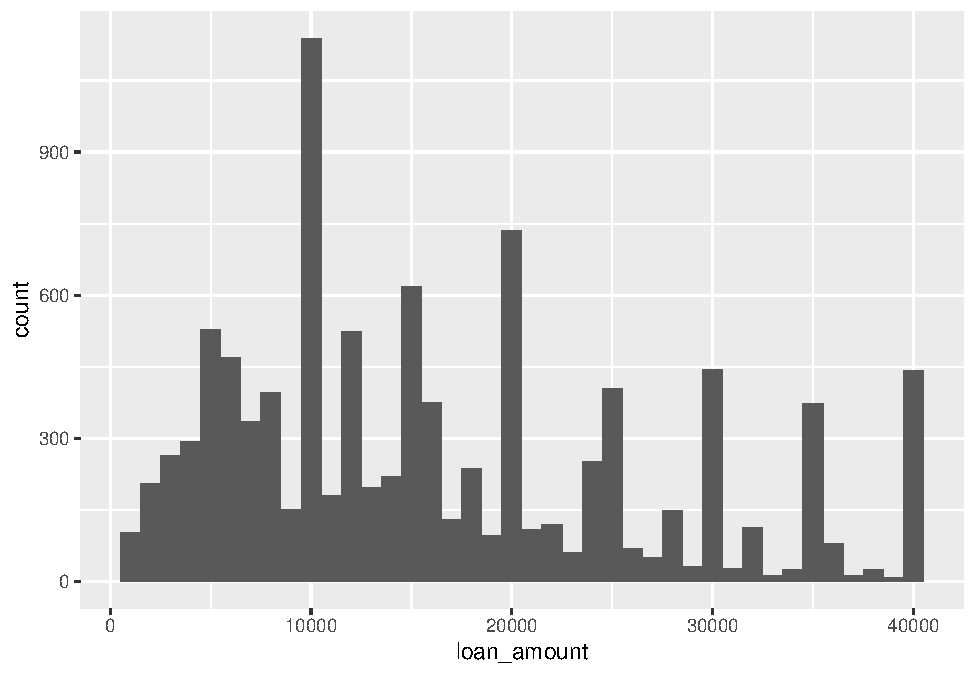
\includegraphics{Challenge-7-File_files/figure-latex/unnamed-chunk-14-1.pdf}

\emph{2. binwidth = 5000}

\begin{Shaded}
\begin{Highlighting}[]
\FunctionTok{ggplot}\NormalTok{(loans) }\SpecialCharTok{+} \FunctionTok{aes}\NormalTok{(}\AttributeTok{x =}\NormalTok{ loan\_amount) }\SpecialCharTok{+}
\FunctionTok{geom\_histogram}\NormalTok{(}\AttributeTok{binwidth =} \DecValTok{5000}\NormalTok{)}
\end{Highlighting}
\end{Shaded}

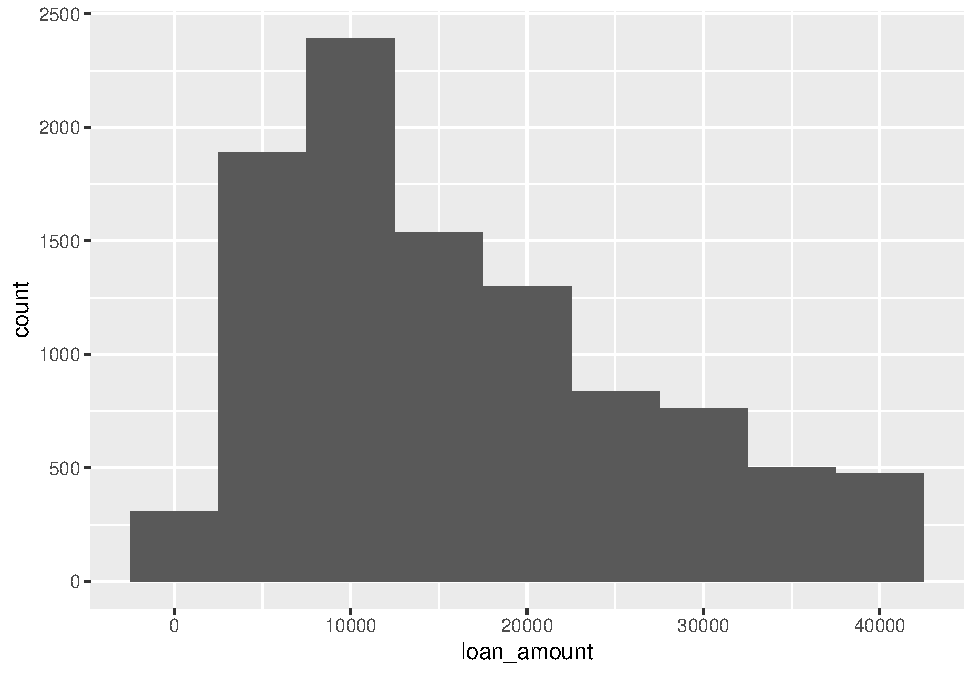
\includegraphics{Challenge-7-File_files/figure-latex/unnamed-chunk-15-1.pdf}

\emph{3. binwidth = 20000}

\begin{Shaded}
\begin{Highlighting}[]
\FunctionTok{ggplot}\NormalTok{(loans) }\SpecialCharTok{+} \FunctionTok{aes}\NormalTok{(}\AttributeTok{x =}\NormalTok{ loan\_amount) }\SpecialCharTok{+}
\FunctionTok{geom\_histogram}\NormalTok{(}\AttributeTok{binwidth =} \DecValTok{20000}\NormalTok{)}
\end{Highlighting}
\end{Shaded}

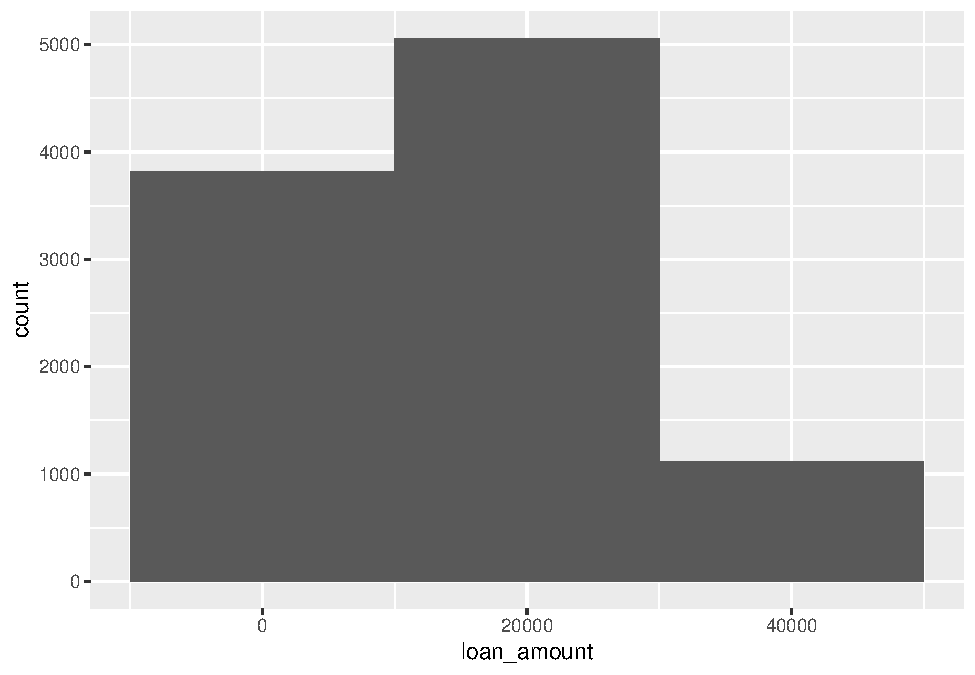
\includegraphics{Challenge-7-File_files/figure-latex/unnamed-chunk-16-1.pdf}

Customizing histograms, with colors and labels

\begin{Shaded}
\begin{Highlighting}[]
\FunctionTok{ggplot}\NormalTok{(loans, }\FunctionTok{aes}\NormalTok{(}\AttributeTok{x =}\NormalTok{ loan\_amount, }\AttributeTok{fill =}\NormalTok{ homeownership)) }\SpecialCharTok{+}
\FunctionTok{geom\_histogram}\NormalTok{(}\AttributeTok{binwidth =} \DecValTok{5000}\NormalTok{, }\AttributeTok{alpha =} \FloatTok{0.5}\NormalTok{) }\SpecialCharTok{+} \FunctionTok{labs}\NormalTok{(}\AttributeTok{x =}\StringTok{"Loan amount ($)"}\NormalTok{,}\AttributeTok{y =}\StringTok{"Frequency"}\NormalTok{,}\AttributeTok{title =}\StringTok{"Amounts of Lending Club loans"}\NormalTok{)}
\end{Highlighting}
\end{Shaded}

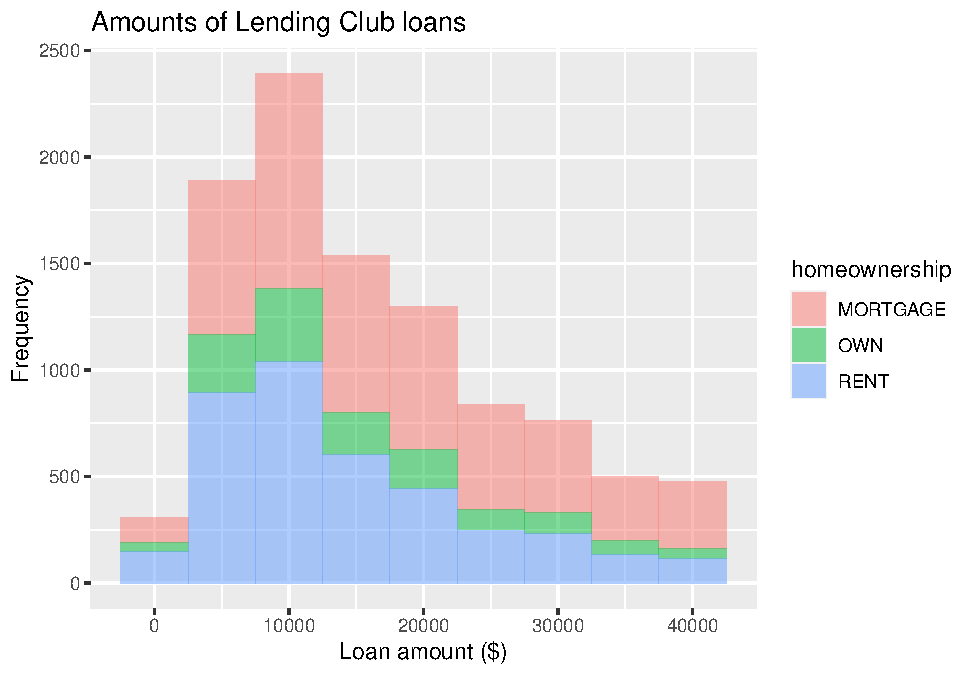
\includegraphics{Challenge-7-File_files/figure-latex/unnamed-chunk-17-1.pdf}

Creating facet plot of histograms with categorical variable

\begin{Shaded}
\begin{Highlighting}[]
\FunctionTok{ggplot}\NormalTok{(loans, }\FunctionTok{aes}\NormalTok{(}\AttributeTok{x =}\NormalTok{ loan\_amount, }\AttributeTok{fill =}\NormalTok{ homeownership)) }\SpecialCharTok{+} \FunctionTok{geom\_histogram}\NormalTok{(}\AttributeTok{binwidth =} \DecValTok{5000}\NormalTok{) }\SpecialCharTok{+} \FunctionTok{labs}\NormalTok{(}\AttributeTok{x =}\StringTok{"Loan amount ($)"}\NormalTok{,}\AttributeTok{y =}
\StringTok{"Frequency"}\NormalTok{,}\AttributeTok{title =}\StringTok{"Amounts of Lending Club loans"}\NormalTok{) }\SpecialCharTok{+}\FunctionTok{facet\_wrap}\NormalTok{(}\SpecialCharTok{\textasciitilde{}}\NormalTok{ homeownership, }\AttributeTok{nrow =}\DecValTok{3}\NormalTok{)}
\end{Highlighting}
\end{Shaded}

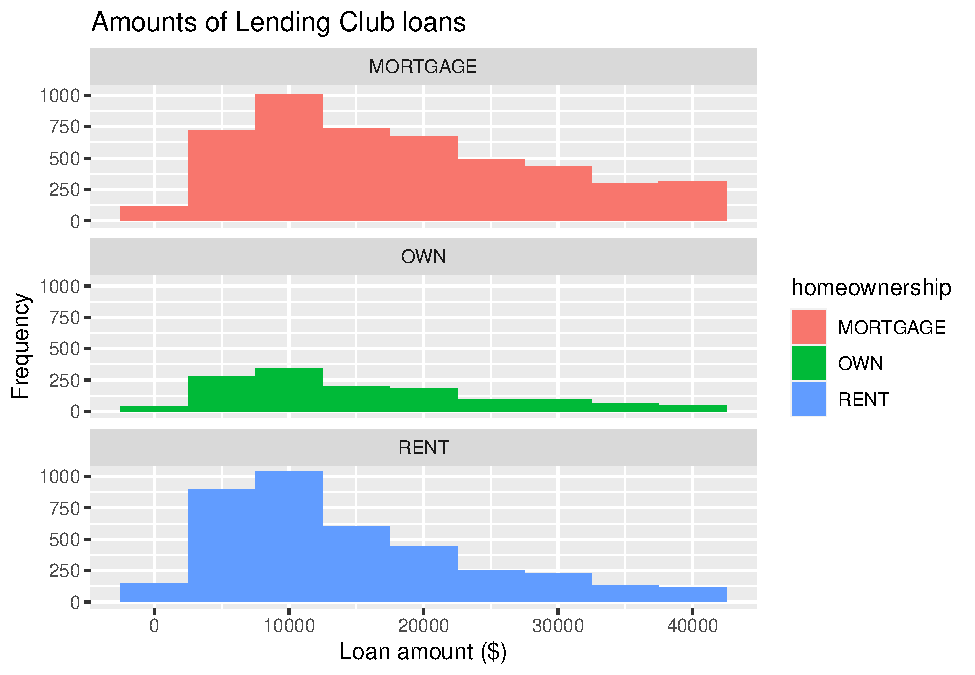
\includegraphics{Challenge-7-File_files/figure-latex/unnamed-chunk-18-1.pdf}

Creating Density Plot with customizable bandwidth

\begin{enumerate}
\def\labelenumi{\arabic{enumi}.}
\tightlist
\item
  Default bandwidth
\end{enumerate}

\begin{Shaded}
\begin{Highlighting}[]
\FunctionTok{ggplot}\NormalTok{(loans, }\FunctionTok{aes}\NormalTok{(}\AttributeTok{x =}\NormalTok{ loan\_amount)) }\SpecialCharTok{+}
\FunctionTok{geom\_density}\NormalTok{(}\AttributeTok{adjust=}\DecValTok{1}\NormalTok{)}
\end{Highlighting}
\end{Shaded}

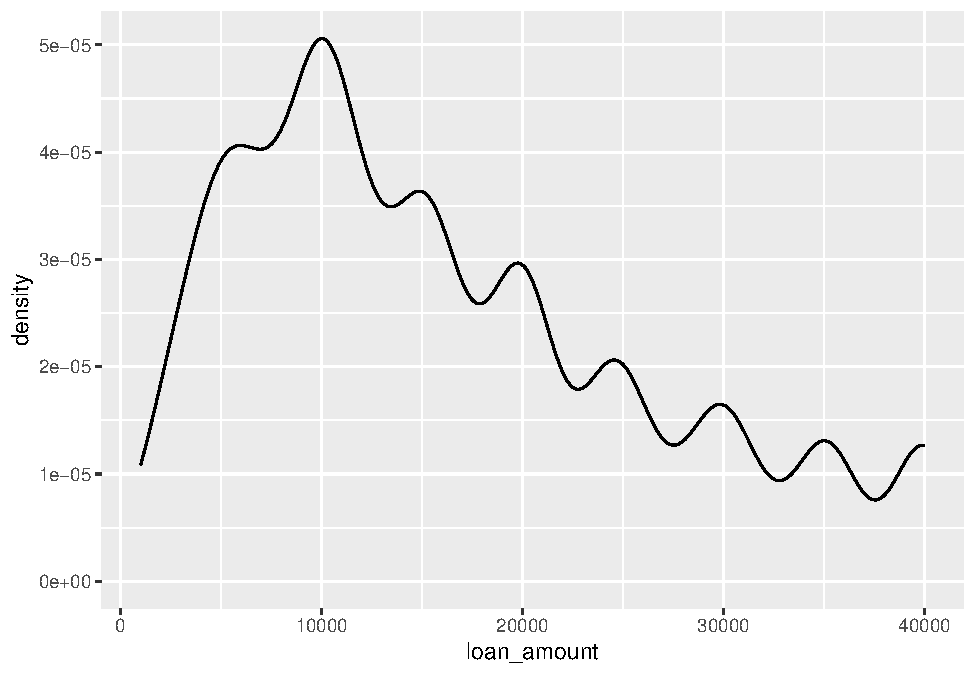
\includegraphics{Challenge-7-File_files/figure-latex/unnamed-chunk-19-1.pdf}

\begin{enumerate}
\def\labelenumi{\arabic{enumi}.}
\setcounter{enumi}{1}
\tightlist
\item
  Increased bandwidth (2)
\end{enumerate}

\begin{Shaded}
\begin{Highlighting}[]
\FunctionTok{ggplot}\NormalTok{(loans, }\FunctionTok{aes}\NormalTok{(}\AttributeTok{x =}\NormalTok{ loan\_amount)) }\SpecialCharTok{+}
\FunctionTok{geom\_density}\NormalTok{(}\AttributeTok{adjust=}\DecValTok{2}\NormalTok{)}
\end{Highlighting}
\end{Shaded}

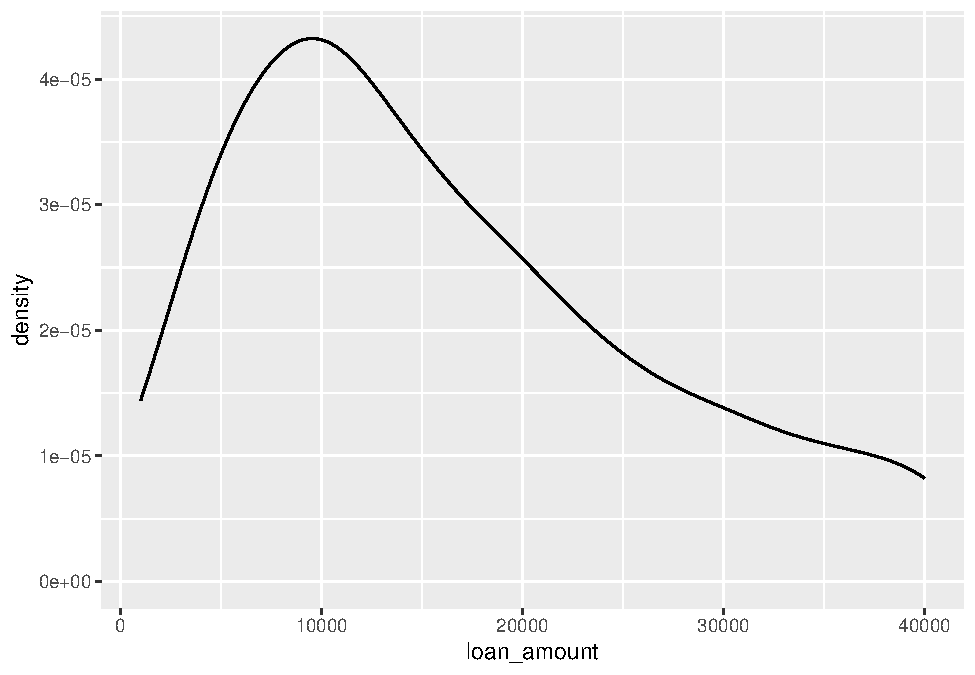
\includegraphics{Challenge-7-File_files/figure-latex/unnamed-chunk-20-1.pdf}

\begin{enumerate}
\def\labelenumi{\arabic{enumi}.}
\setcounter{enumi}{2}
\tightlist
\item
  Decreased bandwidth (0.5)
\end{enumerate}

\begin{Shaded}
\begin{Highlighting}[]
\FunctionTok{ggplot}\NormalTok{(loans, }\FunctionTok{aes}\NormalTok{(}\AttributeTok{x =}\NormalTok{ loan\_amount)) }\SpecialCharTok{+}
\FunctionTok{geom\_density}\NormalTok{(}\AttributeTok{adjust=}\FloatTok{0.5}\NormalTok{)}
\end{Highlighting}
\end{Shaded}

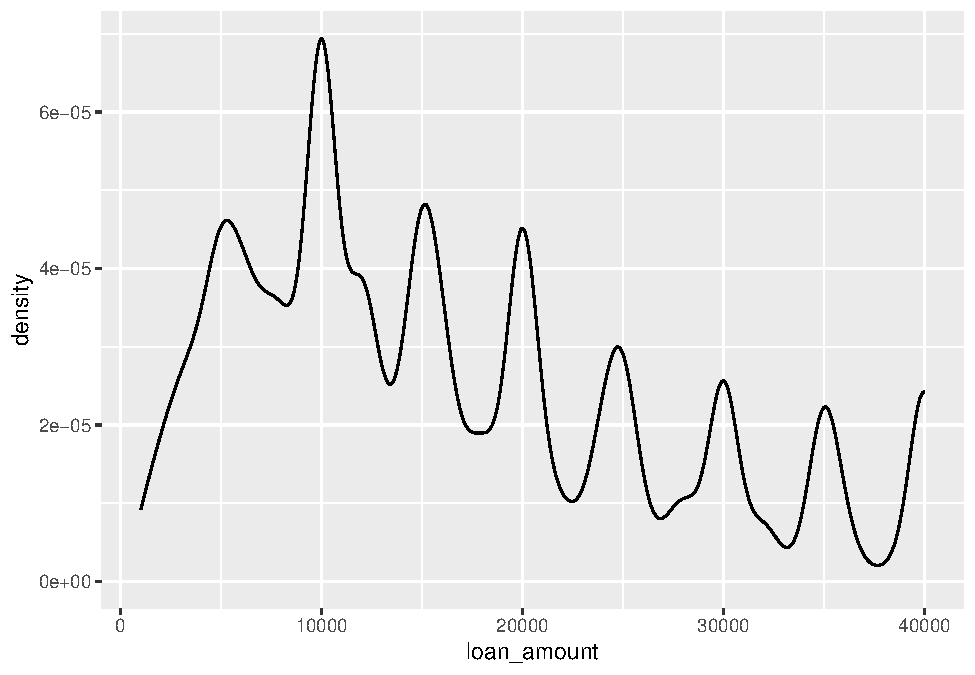
\includegraphics{Challenge-7-File_files/figure-latex/unnamed-chunk-21-1.pdf}

Customizing density plot!

\begin{Shaded}
\begin{Highlighting}[]
\FunctionTok{ggplot}\NormalTok{(loans, }\FunctionTok{aes}\NormalTok{(}\AttributeTok{x =}\NormalTok{ loan\_amount, }\AttributeTok{fill =}\NormalTok{ homeownership)) }\SpecialCharTok{+}
  \FunctionTok{geom\_density}\NormalTok{(}\AttributeTok{adjust =}\DecValTok{2}\NormalTok{, }\AttributeTok{alpha =}\FloatTok{0.5}\NormalTok{) }\SpecialCharTok{+}\FunctionTok{labs}\NormalTok{(}\AttributeTok{x =}\StringTok{"Loan amount ($)"}\NormalTok{,}\AttributeTok{y =}\StringTok{"Density"}\NormalTok{,}\AttributeTok{title =}\StringTok{"Amounts of Lending Club loans"}\NormalTok{, }\AttributeTok{fill =}\StringTok{"Homeownership"}\NormalTok{)}
\end{Highlighting}
\end{Shaded}

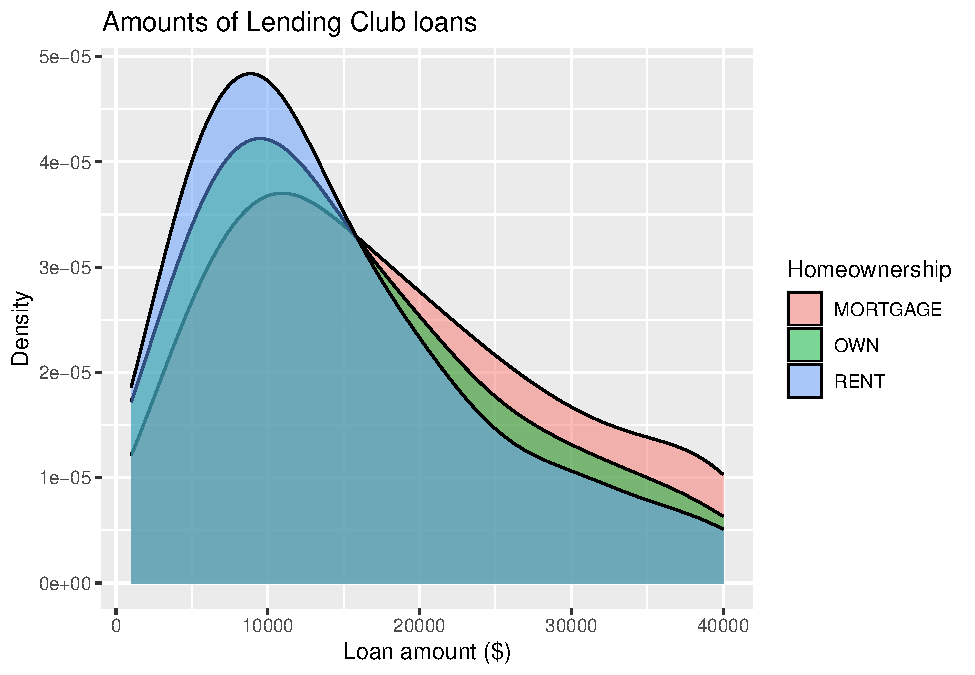
\includegraphics{Challenge-7-File_files/figure-latex/unnamed-chunk-22-1.pdf}
\#\# Plotting box plots

Plotting interest rate of loans

\begin{Shaded}
\begin{Highlighting}[]
\FunctionTok{ggplot}\NormalTok{(loans, }\FunctionTok{aes}\NormalTok{(}\AttributeTok{x =}\NormalTok{ interest\_rate)) }\SpecialCharTok{+}\FunctionTok{geom\_boxplot}\NormalTok{()}
\end{Highlighting}
\end{Shaded}

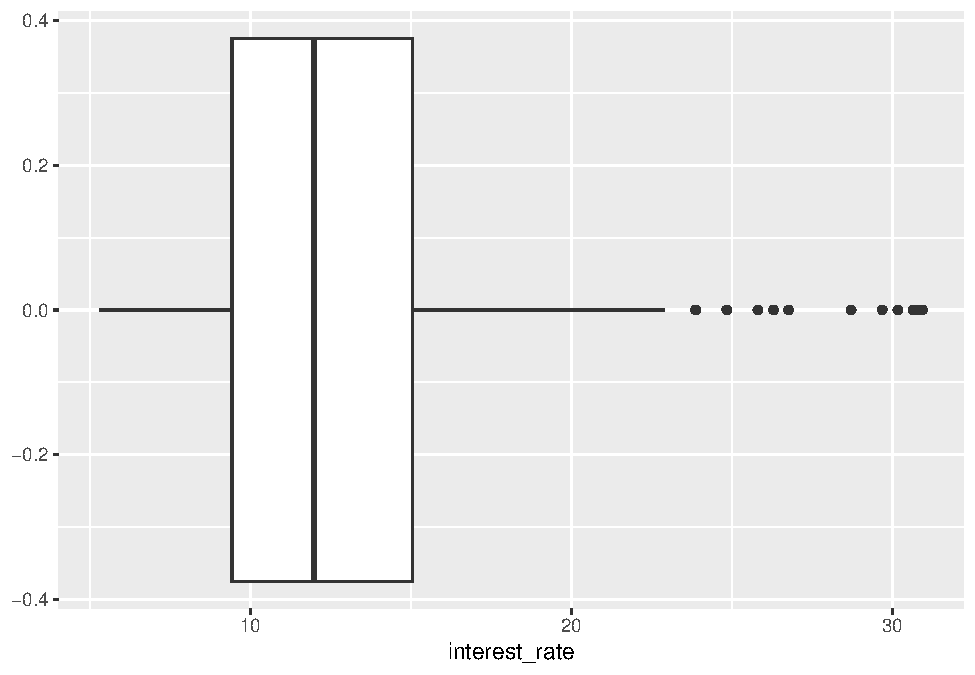
\includegraphics{Challenge-7-File_files/figure-latex/unnamed-chunk-23-1.pdf}

Plotting annual income against loans

\begin{Shaded}
\begin{Highlighting}[]
\FunctionTok{ggplot}\NormalTok{(loans, }\FunctionTok{aes}\NormalTok{(}\AttributeTok{x =}\NormalTok{ annual\_income)) }\SpecialCharTok{+}
\FunctionTok{geom\_boxplot}\NormalTok{()}
\end{Highlighting}
\end{Shaded}

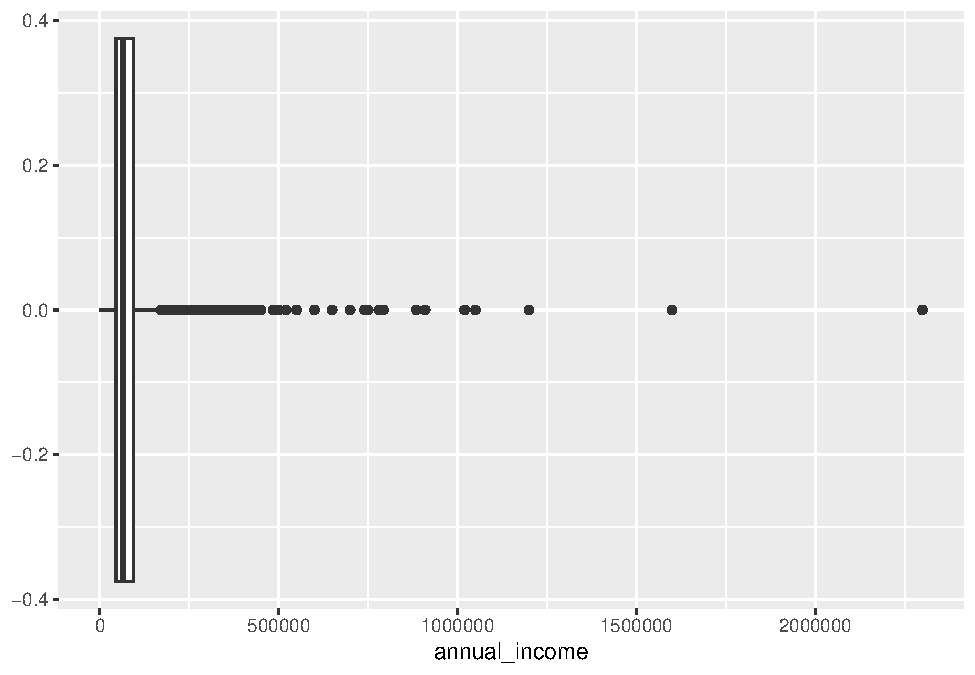
\includegraphics{Challenge-7-File_files/figure-latex/unnamed-chunk-24-1.pdf}
Customizing box plots

\begin{Shaded}
\begin{Highlighting}[]
\FunctionTok{ggplot}\NormalTok{(loans, }\FunctionTok{aes}\NormalTok{(}\AttributeTok{x =}\NormalTok{ interest\_rate)) }\SpecialCharTok{+}\FunctionTok{geom\_boxplot}\NormalTok{() }\SpecialCharTok{+}\FunctionTok{labs}\NormalTok{(}\AttributeTok{x =}\StringTok{"Interest rate (\%)"}\NormalTok{,}\AttributeTok{y =}\ConstantTok{NULL}\NormalTok{,}\AttributeTok{title =}\StringTok{"Interest rates of Lending Club loans"}\NormalTok{) }\SpecialCharTok{+}\FunctionTok{theme}\NormalTok{( }\AttributeTok{axis.ticks.y =} \FunctionTok{element\_blank}\NormalTok{(), }\AttributeTok{axis.text.y =} \FunctionTok{element\_blank}\NormalTok{() )}
\end{Highlighting}
\end{Shaded}

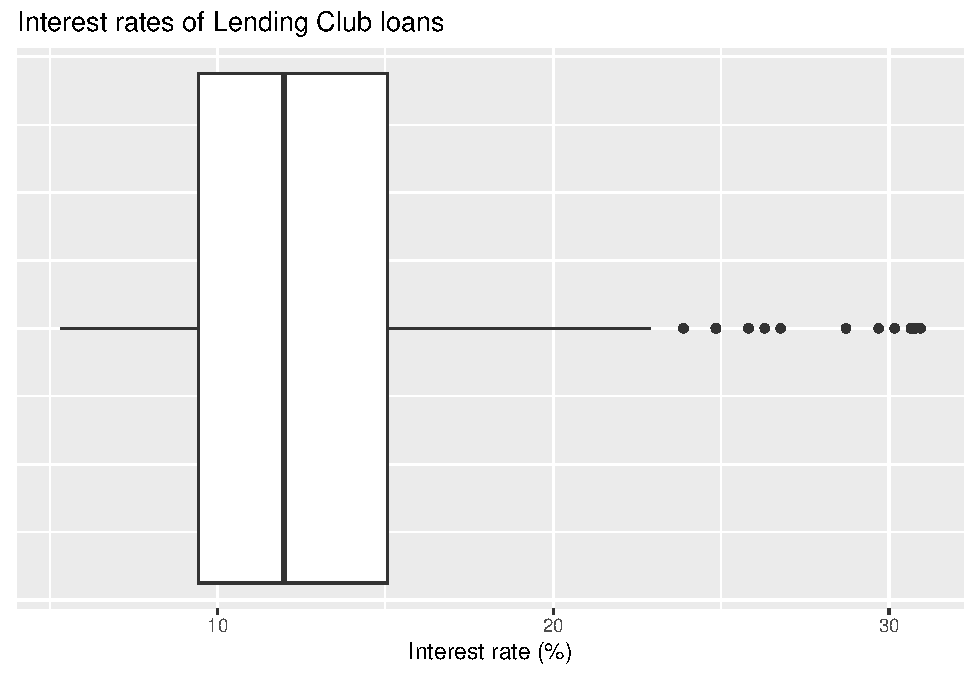
\includegraphics{Challenge-7-File_files/figure-latex/unnamed-chunk-25-1.pdf}

By grade of loan

\begin{Shaded}
\begin{Highlighting}[]
\FunctionTok{ggplot}\NormalTok{(loans, }\FunctionTok{aes}\NormalTok{(}\AttributeTok{x =}\NormalTok{ interest\_rate,}\AttributeTok{y =}\NormalTok{ grade)) }\SpecialCharTok{+}\FunctionTok{geom\_boxplot}\NormalTok{() }\SpecialCharTok{+}\FunctionTok{labs}\NormalTok{(}\AttributeTok{x =}
\StringTok{"Interest rate (\%)"}\NormalTok{,}\AttributeTok{y =}\StringTok{"Grade"}\NormalTok{,}\AttributeTok{title =}\StringTok{"Interest rates of Lending Club loans"}\NormalTok{,}\AttributeTok{subtitle=} \StringTok{"by grade of loan"}\NormalTok{)}
\end{Highlighting}
\end{Shaded}

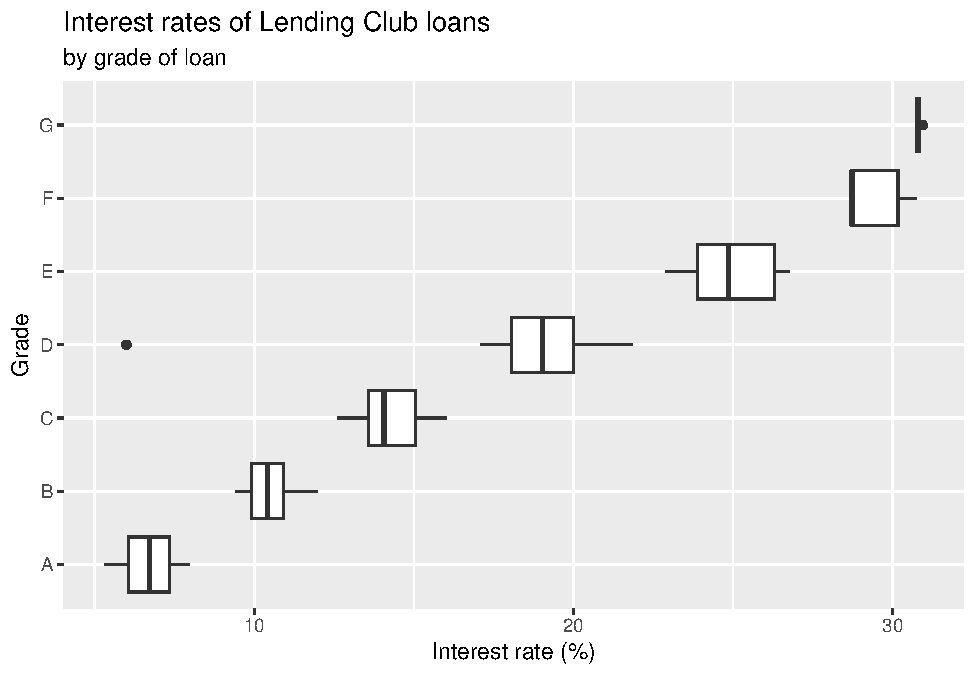
\includegraphics{Challenge-7-File_files/figure-latex/unnamed-chunk-26-1.pdf}

\hypertarget{creating-scatterplot}{%
\subsection{Creating Scatterplot}\label{creating-scatterplot}}

\begin{Shaded}
\begin{Highlighting}[]
\FunctionTok{ggplot}\NormalTok{(loans, }\FunctionTok{aes}\NormalTok{(}\AttributeTok{x =}\NormalTok{ debt\_to\_income, }\AttributeTok{y =}\NormalTok{ interest\_rate)) }\SpecialCharTok{+}
\FunctionTok{geom\_point}\NormalTok{()}
\end{Highlighting}
\end{Shaded}

\begin{verbatim}
## Warning: Removed 24 rows containing missing values (`geom_point()`).
\end{verbatim}

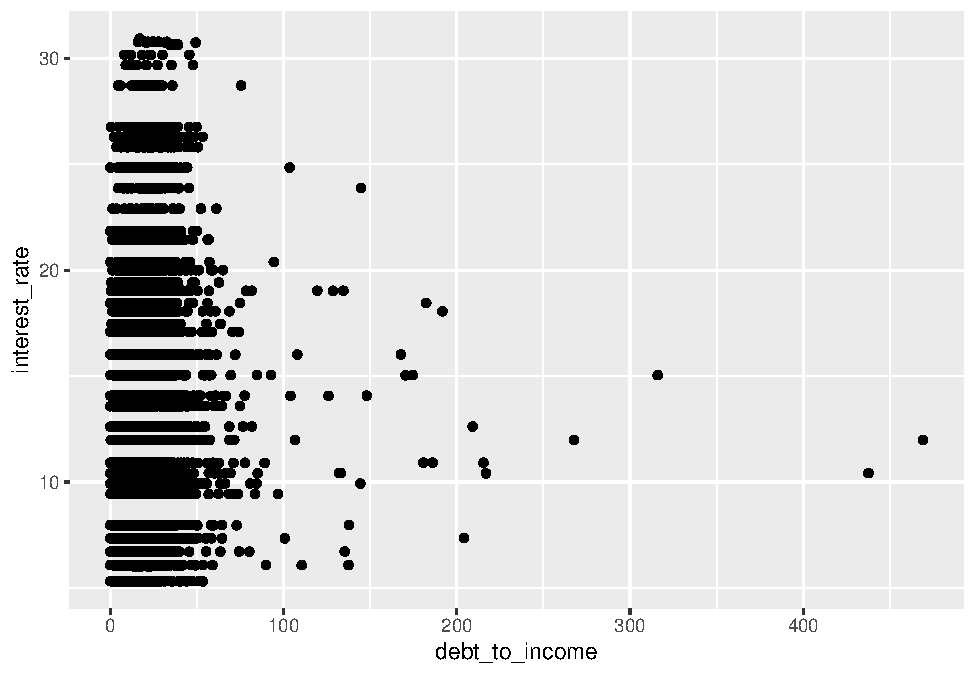
\includegraphics{Challenge-7-File_files/figure-latex/unnamed-chunk-27-1.pdf}

\hypertarget{creating-hex-plot}{%
\subsection{Creating Hex Plot}\label{creating-hex-plot}}

\begin{Shaded}
\begin{Highlighting}[]
\FunctionTok{ggplot}\NormalTok{(loans }\SpecialCharTok{\%\textgreater{}\%} \FunctionTok{filter}\NormalTok{(debt\_to\_income }\SpecialCharTok{\textless{}}\DecValTok{100}\NormalTok{),}\FunctionTok{aes}\NormalTok{(}\AttributeTok{x =}\NormalTok{ debt\_to\_income, }\AttributeTok{y =}\NormalTok{ interest\_rate)) }\SpecialCharTok{+}\FunctionTok{geom\_hex}\NormalTok{()}
\end{Highlighting}
\end{Shaded}

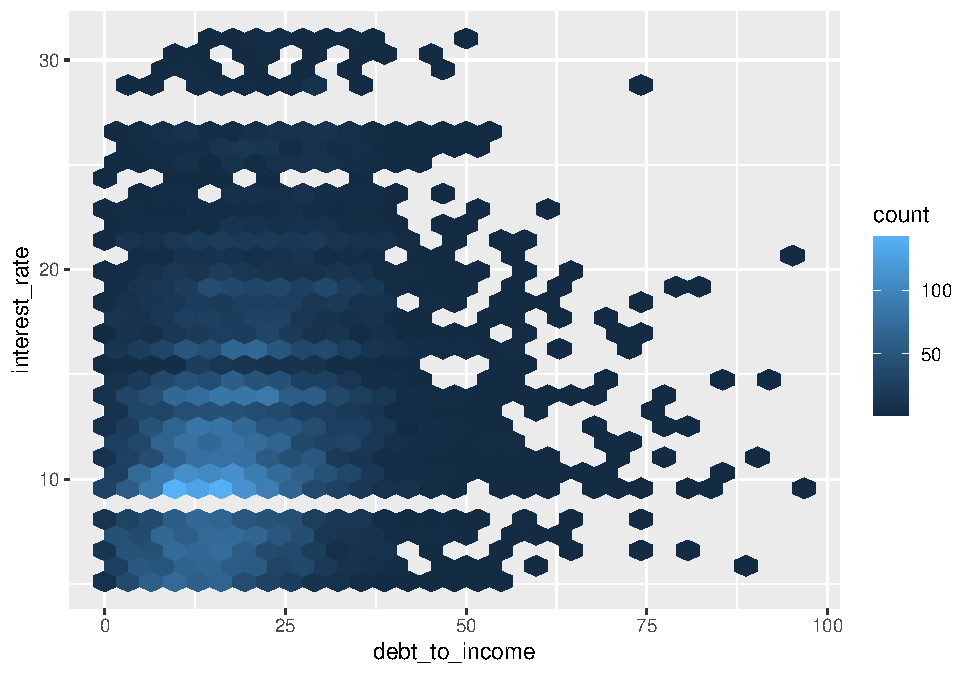
\includegraphics{Challenge-7-File_files/figure-latex/unnamed-chunk-28-1.pdf}

\hypertarget{creating-bar-plot}{%
\subsection{Creating Bar Plot}\label{creating-bar-plot}}

\begin{Shaded}
\begin{Highlighting}[]
\FunctionTok{ggplot}\NormalTok{(loans, }\FunctionTok{aes}\NormalTok{(}\AttributeTok{x =}\NormalTok{ homeownership)) }\SpecialCharTok{+}\FunctionTok{geom\_bar}\NormalTok{()}
\end{Highlighting}
\end{Shaded}

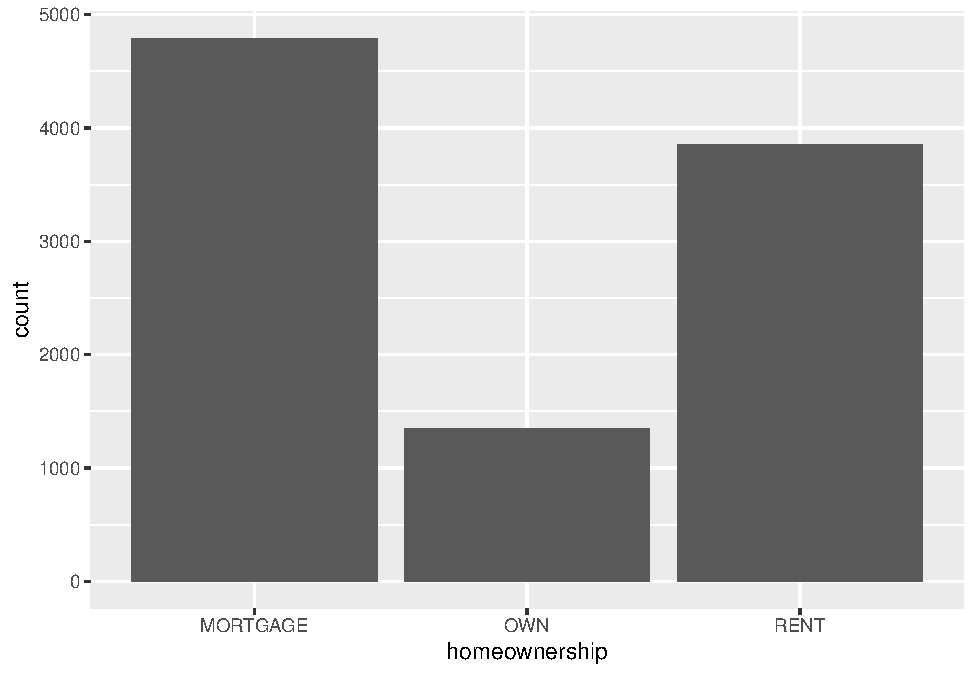
\includegraphics{Challenge-7-File_files/figure-latex/unnamed-chunk-29-1.pdf}

Customizing segmented bar plot (by grade of homeownership)

\begin{Shaded}
\begin{Highlighting}[]
\FunctionTok{ggplot}\NormalTok{(loans, }\FunctionTok{aes}\NormalTok{(}\AttributeTok{x =}\NormalTok{ homeownership,}
\AttributeTok{fill =}\NormalTok{ grade)) }\SpecialCharTok{+}
\FunctionTok{geom\_bar}\NormalTok{()}
\end{Highlighting}
\end{Shaded}

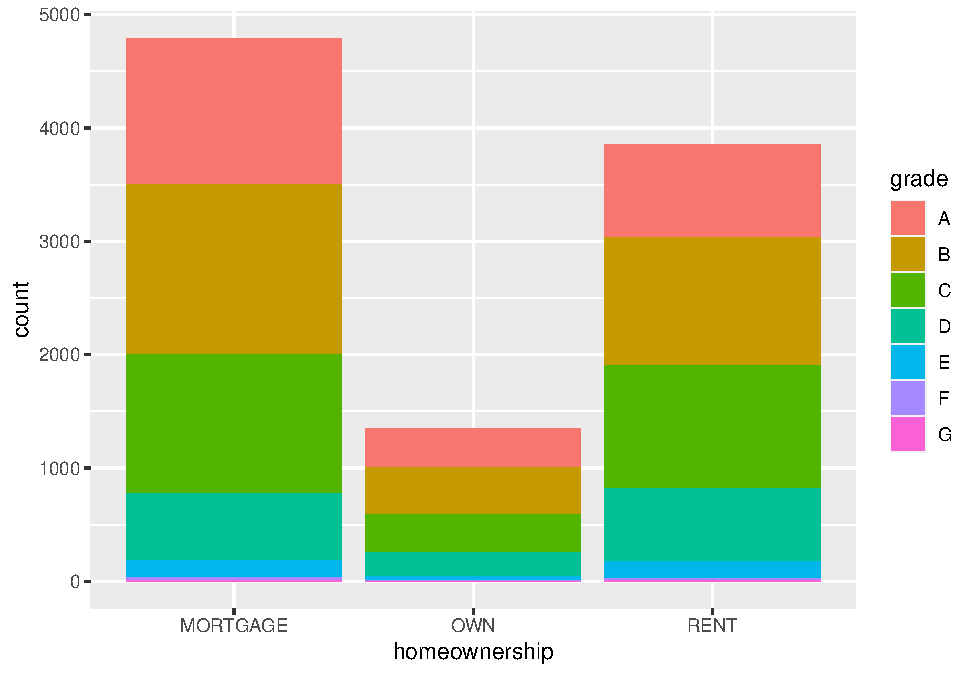
\includegraphics{Challenge-7-File_files/figure-latex/unnamed-chunk-30-1.pdf}

Customizing bar plots (by proportion)

\begin{Shaded}
\begin{Highlighting}[]
\FunctionTok{ggplot}\NormalTok{(loans, }\FunctionTok{aes}\NormalTok{(}\AttributeTok{y =}\NormalTok{ homeownership, }\AttributeTok{fill =}\NormalTok{ grade)) }\SpecialCharTok{+} \FunctionTok{geom\_bar}\NormalTok{(}\AttributeTok{position =}
\StringTok{"fill"}\NormalTok{) }\SpecialCharTok{+}\FunctionTok{labs}\NormalTok{( }\AttributeTok{x =}\StringTok{"Proportion"}\NormalTok{, }\AttributeTok{y =}\StringTok{"Homeownership"}\NormalTok{, }\AttributeTok{fill =}\StringTok{"Grade"}\NormalTok{, }\AttributeTok{title =}\StringTok{"Grades of Lending Club loans"}\NormalTok{, }\AttributeTok{subtitle=}\StringTok{"and homeownership of lendee"}\NormalTok{)}
\end{Highlighting}
\end{Shaded}

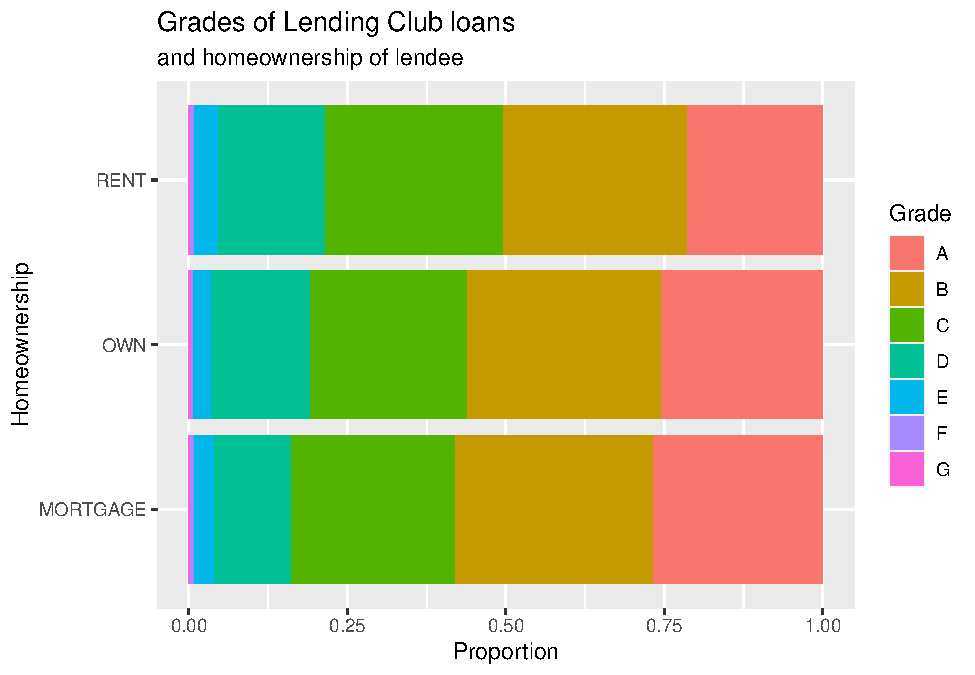
\includegraphics{Challenge-7-File_files/figure-latex/unnamed-chunk-31-1.pdf}

\hypertarget{creating-violin-plots}{%
\subsection{Creating violin plots}\label{creating-violin-plots}}

\begin{Shaded}
\begin{Highlighting}[]
\FunctionTok{ggplot}\NormalTok{(loans, }\FunctionTok{aes}\NormalTok{(}\AttributeTok{x =}\NormalTok{ homeownership, }\AttributeTok{y =}\NormalTok{ loan\_amount)) }\SpecialCharTok{+}
\FunctionTok{geom\_violin}\NormalTok{()}
\end{Highlighting}
\end{Shaded}

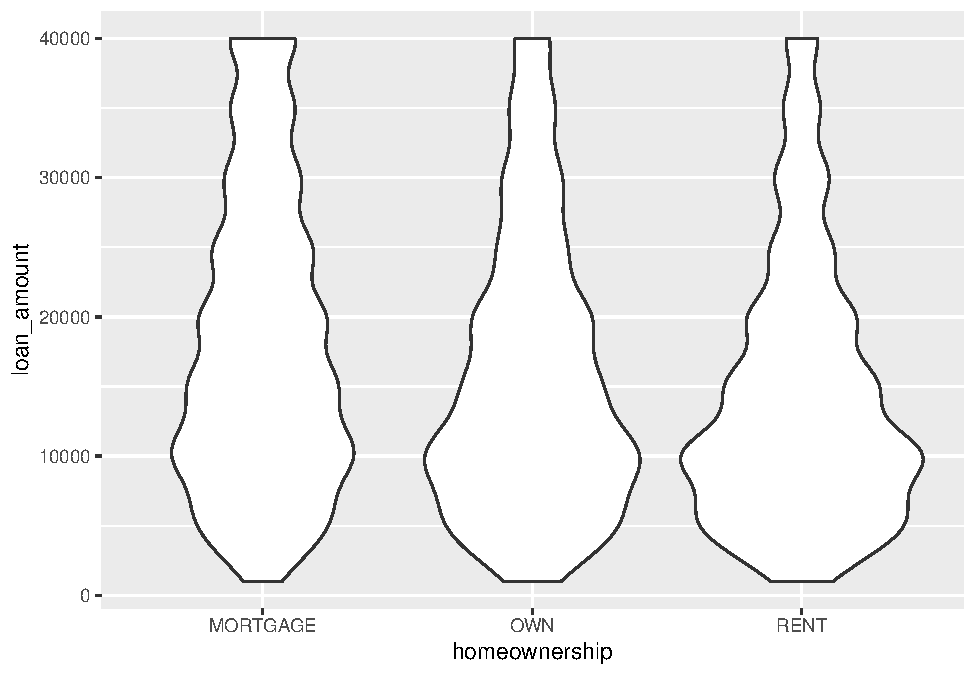
\includegraphics{Challenge-7-File_files/figure-latex/unnamed-chunk-32-1.pdf}

\hypertarget{creating-ridge-plots}{%
\subsection{Creating ridge plots}\label{creating-ridge-plots}}

\begin{Shaded}
\begin{Highlighting}[]
\FunctionTok{library}\NormalTok{(ggridges)}
\end{Highlighting}
\end{Shaded}

\begin{verbatim}
## Warning: package 'ggridges' was built under R version 4.2.3
\end{verbatim}

\begin{Shaded}
\begin{Highlighting}[]
\FunctionTok{ggplot}\NormalTok{(loans, }\FunctionTok{aes}\NormalTok{(}\AttributeTok{x =}\NormalTok{ loan\_amount, }\AttributeTok{y =}\NormalTok{ grade, }\AttributeTok{fill =}\NormalTok{ grade, }\AttributeTok{color =}\NormalTok{ grade)) }\SpecialCharTok{+}\FunctionTok{geom\_density\_ridges}\NormalTok{(}\AttributeTok{alpha =}\FloatTok{0.5}\NormalTok{)}
\end{Highlighting}
\end{Shaded}

\begin{verbatim}
## Picking joint bandwidth of 2360
\end{verbatim}

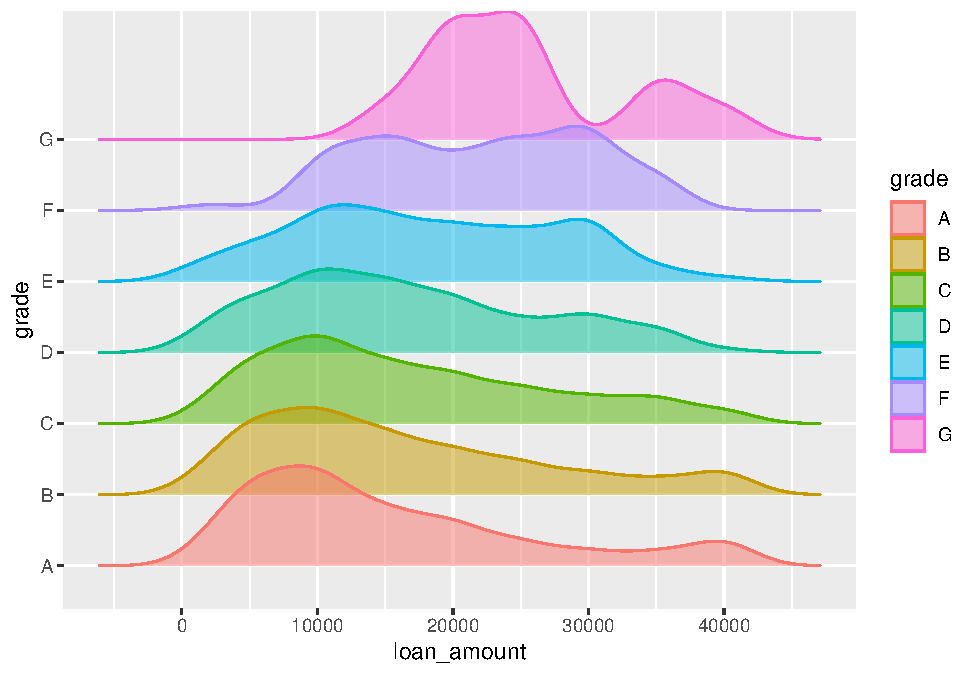
\includegraphics{Challenge-7-File_files/figure-latex/unnamed-chunk-33-1.pdf}

Thank you!

\end{document}
